% !Mode:: "TeX:UTF-8"
%%%%%%%%%%%%%%%%%%%%%%%%%%%%%%%%%%%%%%%%%%%%%%%%%%%%%%%%%%%%%%%%%%%%%%%%%%%%%%%%
%
%                          大工至善,大学至臻
%
%                        哈尔滨工程大学论文模板
%
%                      Email: lwh@hrbeu.edu.cn
%                      https://www.hrbeu.edu.cn
%
%                  https://gitee.com/liwenhui/heuthesis
%
%%%%%%%%%%%%%%%%%%%%%%%%%%%%%%%%%%%%%%%%%%%%%%%%%%%%%%%%%%%%%%%%%%%%%%%%%%%%%%%%
\documentclass[type=doctor,fontset=windows]{heuthesisbook}
% 此处选项中不要有空格
%%%%%%%%%%%%%%%%%%%%%%%%%%%%%%%%%%%%%%%%%%%%%%%%%%%%%%%%%%%%%%%%%%%%%%%%%%%%%%%%
% 必填选项
% type=doctor|master|bachelor|postdoc
%%%%%%%%%%%%%%%%%%%%%%%%%%%%%%%%%%%%%%%%%%%%%%%%%%%%%%%%%%%%%%%%%%%%%%%%%%%%%%%%
% 选填选项(选填选项的缺省值已经尽可能满足了大多数需求,除非明确知道自己有什么
% 需求)
% tocfour=true|false
%   含义:是否添加第四级目录,只对本科文科个别要求四级目录有效,缺省值为
%   false
% fontset=windows|mac|ubuntu|fandol|adobe
%   含义:设置字体,默认情况会自动识别系统,然后设置字体。后两个是开源字体,自行
%   下载安装后设置使用。
% subtitle=true|false
%   含义:论文题目是否含有副标题,缺省值为false,如果有要在cover中设置副标
%   题内容,封面中显示。
% openright=true|false
%   含义:博士论文是否要求章节首页必须在奇数页,此选项不在规范要求中,按个
%   人喜好自行决定。 默认否。注意,我校的默认情况是打印版博士论文要求右翻页
%   ,电子版要求非右翻页且无空白页。如果想DIY(或身不由己DIY)在什么地方右
%   翻页,将这个选项设置为false,然后在目标位置添加`\cleardoublepage`命令即
%   可。
% pageempty=true|false
%   含义:空白页是否无页眉页脚(默认否)。
%%%%%%%%%%%%%%%%%%%%%%%%%%%%%%%%%%%%%%%%%%%%%%%%%%%%%%%%%%%%%%%%%%%%%%%%%%%%%%%%
\usepackage{heuthesis}

\graphicspath{{figures/}}

\begin{document}
\frontmatter
% !Mode:: "TeX:UTF-8"

\heusetup{
  %******************************
  % 注意:
  %   1. 配置里面不要出现空行
  %   2. 不需要的配置信息可以删除
  %******************************
  %
  %=========
  % 秘级编号
  %=========
  statesecrets={公开},          %密级
  cnumber={no9527},             %编号
  natclassifiedindex={TM301.2}, %分类号
  intclassifiedindex={62-5},    %UDC编号
  %
  %=========
  % 中文信息
  %=========
  ctitlecover={基于~\LaTeX~的哈尔滨工程大学本硕博\\论文模板使用说明}, %放在封面中使用,在需要换行的地方插入\\
  ctitle={基于~\LaTeX~的哈尔滨工程大学本硕博论文模板使用说明},        %页眉使用论文标题,不换行
  csubject={动力工程及工程热物理}, %专业
  caffil={动力与能源工程学院},     %所在单位/学院
  cauthor={马冬梅},                %论文作者
  csupervisor={孔夫子},            %指导老师
  cprofessional={教授},            %指导老师职称
  csupervisorcaffil={动力与能源工程学院}, %导师单位
  % 日期自动使用当前时间,若需指定按如下方式修改:
  %cdate={超新星纪元}, %封面日期,不指定使用当前日期
  csubmitdate={20XX年XX月}, %提交日期
  coralexdate={20XX年XX月}, %答辩日期
  cstudentid={202103123},   %学号
  %
  %=========
  % 英文信息
  %=========
  etitle={Manual of~ \LaTeX ~Thesis Template of\\ Harbin Engineering University}, %论文题目(英文),在需要换行的地方插入\\
  %
  % 中英文关键词,用“英文逗号(,)”分割
  ckeywords={\TeX, \LaTeX, 论文, 模板},
  ekeywords={\TeX, \LaTeX, template, thesis},
}

\begin{cabstract}
  摘要的字数(以汉字计),本科、硕士学位论文一般为500 $\sim$ 1000字,博士学位论文为1000 $\sim$ 2000字,
  均以能将规定内容阐述清楚为原则,文字要精练,段落衔接要流畅。摘要页不需写出论文题目。
  英文摘要与中文摘要的内容应一致,在语法、用词上应准确无误,语言简练通顺。

  关键词是为了文献标引工作、用以表示全文主要内容信息的单词或术语。关键词不超过 5
  个,每个关键词中间用分号分隔。(关键词分隔符不用考虑,模板会自动处理。英文关键词同理。)
\end{cabstract}

\begin{eabstract}
  An abstract of a dissertation is a summary and extraction of research work
  and contributions. Included in an abstract should be description of research
  topic and research objective, brief introduction to methodology and research
  process, and summarization of conclusion and contributions of the
  research. An abstract should be characterized by independence and clarity and
  carry identical information with the dissertation. It should be such that the
  general idea and major contributions of the dissertation are conveyed without
  reading the dissertation.

  An abstract should be concise and to the point. It is a misunderstanding to
  make an abstract an outline of the dissertation and words “the first
  chapter”, “the second chapter” and the like should be avoided in the
  abstract.

  Key words are terms used in a dissertation for indexing, reflecting core
  information of the dissertation. An abstract may contain a maximum of 5 key
  words, with semi-colons used in between to separate one another.
\end{eabstract}

 % 封面和扉页
\makecover

\authorization               % 使用模板生成的原始原创性与授权声明页
%%\authorization[auscan.pdf] % 使用签字扫描版的原创性与授权声明页

\cleardoublepage   % 控制右开页,与前文连续开页时注释掉
\makeabstract      % 封面和摘要

\cleardoublepage   % 控制右开页,与前文连续开页时注释掉
\tableofcontents   % 论文目录

%%\cleardoublepage % 控制右开页,与前文连续开页时注释掉
\listoffigures     % 插图目录, 如不需要可用 % 注释掉下面两行

%%\cleardoublepage % 控制右开页,与前文连续开页时注释掉
\listoftables      % 表格目录, 如不需要可用 % 注释掉下面两行

%%----------  论文主体,可以根据需要添加章节 --------------
\cleardoublepage % 控制右开页,后续论文正文一般采用此格式
\mainmatter
%! TEX program = xelatex
%! TEX root = ../main.tex
%! TEX encoding = utf-8

%%%%%%%%%%%%%%%%%%%%%%%%%%%%%%%%%%%%%%%%%%%%%%%%%%%%%%%%%%%%%%%%%%%%%%
%
%  哈尔滨工程大学学位论文 XeLaTeX 模版 —— 正文文件 chap01.tex
%
%  版本:1.0.0
%  最后更新:
%  修改者:Leo LiWenhui lwh@hrbeu.edu.cn
%  修订者:
%  编译环境1:Ubuntu 12.04 + TeXLive 2013/2014
%  编译环境2:Windows 7/8  + TeXLive 2013/2014
%
%%%%%%%%%%%%%%%%%%%%%%%%%%%%%%%%%%%%%%%%%%%%%%%%%%%%%%%%%%%%%%%%%%%%%

%% 如需英文目录,章节的定义需要改用\BiChapterhe和\BiSection等, 例如
%%   \BiChapter{中文章名称}{Chapter Name In English}
%%   \BiSection{中文节名称}{Section Name In English}
%%   \BiSubSection{中文小节名称}{SubSection Name In English}

\chapter{绪论}
\label{chap01}

\section{引言}

学位论文是典型的科技文献,其具有规范的科技文献排版要求,特别是理工类学位论文需要大量的公式和文档排版。因此研究如何提高学位论文编辑排版工作的效率有非常重要的现实意义。本文结合\XeLaTeX{}\footnote{读音:拉泰赫}文档编辑的特点,将Xe\LaTeX{}用在学位论文编辑排版,使用这种方法可以提高论文编辑的效率与排版质量,最大程度地降低论文排版的繁琐性。

\XeLaTeX{}是一种专业的科技文献排版语言,使用它写文档具有如下优势:
\begin{itemize}
  \item 将内容与格式分离,使人专注于内容书写;
  \item 编程化控制排版格式,工作灵活性和精确度高;
  \item 跨平台,兼容性和稳定性非常好。
\end{itemize}

本模板是在参考其他学校论文模板的基础上,根据哈尔滨工程的大学研究生院对本科与研究生论文的格式要求制作,通过此模板,所有排版格式化工作由模板完成,使用户集中于论文的内容上。

\section{TeX~简介}

谈到\TeX{},人们首先会想起Donald E. Knuth \footnote{1960年凯斯工学院数学学士,1963年加州理工数学博士,同年留校任教。1968年跳槽到斯坦福,1974年获图灵奖,1992年退休,1995年获冯·诺依曼奖。}(1938--)。1962年Knuth开始写一本关于编译器设计的书,原计划是12章的单行本。不久Knuth觉得此书涉及的领域应该扩大,于是越写越多,一发不可收拾。1965年完成的初稿居然有3000页,据出版商估计,这些手稿印刷出来大概需要2000页。出书的计划只好改为七卷,每卷一或两章,这就是 \emph{The Art of Computer Programming} \footnote{已完成的前三卷是:\emph{Fundamental Algorithms}, \emph{Seminumerical Algorithms}, \emph{Sorting and Searching}。 第四卷 \emph{Combinatorial Algorithms} 的第一部分4A已出版,其余部分和第五卷 \emph{Syntactic Algorithms}正在写作中,预计2020年完成。第六卷 \emph{Theory of Context-free Languages}和第七卷 \emph{Compiler Techniques}尚未安排上工作日程。}。

1976年,当Knuth改写第二卷的第二版时,很郁闷地发现第一卷的铅版不见了;而当时数字排版刚刚兴起,质量还差强人意。于是Knuth决定自己开发一个全新的排版系统,这就是 \TeX。

1978年 \TeX 第一版发布后好评如潮,Knuth趁热打铁在1982年发布了第二版,1989年发布的 \TeX{} 3.0将7位字符改为8位。之后Knuth宣布除了修正漏洞停止 \TeX 的开发,因为它已经很稳定,而且他要集中精力完成那部巨著的后几卷。

从那时起,每发布一个修正版,版本号就增加一位小数,趋近于$\pi$;当前版本是2008年的3.1415926。他的另一个软件METAFONT的版本号趋近于$e$,目前是2.718281。Knuth希望在他离世时,\TeX 和METAFONT的版本号永远固定下来,从此人们不再改动他的代码。

\subsection{格式}

\TeX 是一种语言也是一个排版引擎 (engine) ,引擎的基本功能就是把字排成行,把行排成页,涉及到断字、断行、分页等算法。基本的 \TeX 系统只有300多个元命令 (primitive) ,十分精悍,但是很难读懂,只适于非正常人类。所以Knuth提供了一种格式 (format,宏命令的集合) 对 \TeX 进行了封装,这就是Plain \TeX ,包含600多个宏命令,然而它还是不够高级。

1980年代初期,斯坦福研究所的Leslie Lamport (1941--)\footnote{1970年加入麻省计算机同伙公司。2008年获冯·诺依曼奖。} 开发了一种新的格式,也就是 \LaTeX。1992年 \LaTeX{} 2.09发布后,Lamport退居二线,之后的开发活动由Frank Mittelbach 等人接管。他们发布的最后版本是1994年的 \LaTeXe,\LaTeX 3 的开发也在进行中,只是正式版看起来遥遥无期。

\subsection{宏包}

\LaTeX 出现之后,在它的基础上出现了很多宏包 (package) 。起初,美国数学学会 {} 看着 \TeX 是好的,就派Michael D. Spivak (1940--)\footnote{1964年普林斯顿数学博士。} 开发基于Plain \TeX 的宏包AmS\TeX{},它的开发进行了两年 (1983--1985) 。后来与时俱进的AMS又看着 \LaTeX 是好的,就想转移阵地,但是他们的字体遇到了麻烦。

恰好Mittelbach和Rainer Schöpf\footnote{\LaTeX 3的开发者之一。} 刚刚搞了个字体系统new font selection scheme for \LaTeX{} (NFSS) ,AMS看着还不错,就拜托他们把AMSFonts加入 \LaTeX,继而在1989年请他们开发\AmS\LaTeX{}。次年\AmS\LaTeX 正式发布,之后它被整合为 \AmS 宏包。

\section{优点缺点}

通过上节内容我们已经知道,\TeX 相对于其他标记语言有较大优势,但是在桌面印刷领域还有一种不可忽视的类别,所见即所得 (WYSIWYG) 系统,比如微软的Word。其实Word也有自己的域代码 (field code) ,只是一般用户不太了解。

一般而言,\TeX 相对于所见即所得系统有如下优点:
\begin{itemize}
  \item  高质量,它制作的版面看起来更专业,数学公式尤其赏心悦目。
  \item  结构化,它的文档结构清晰。
  \item  批处理,它的源文件是文本文件,便于批处理,虽然解释 (parse) 源文件可能很费劲。
  \item  跨平台,它几乎可以运行于所有电脑硬件和操作系统平台。
  \item  免费,多数 \TeX 软件都是免费的,虽然也有一些商业软件。
\end{itemize}

相应地,\TeX 由于其工作流程,设计原则,资源的缺乏,以及历史局限性等原因也存在一些缺陷:
\begin{itemize}
  \item  语法不如HTML和XML严谨、清晰。
  \item  制作过程繁琐,有时需要反复编译,不能直接或实时看到结果。
  \item  宏包鱼龙混杂,水准参差不齐,风格不够统一。
  \item  排版样式比较统一,但因而缺乏灵活性。
  \item  相对于商业软件,用户支持不够好,文档不完善。
\end{itemize}


\section{XeTeX简介}

\XeTeX{}\footnote{英文发音为"zee-\TeX{}"}是一种使用Unicode的\TeX{}排版引擎,并支持一些现代字体技术,例如OpenType。其作者和维护者是Jonathan Kew,并以X11自由软件许可证发布。

虽然\XeTeX{}最初只是为Mac OS X所开发,但它现在在各主要平台上都可以运作。它原生的支持Unicode,并默认其输入文件为UTF-8编码。\XeTeX{}可以在不进行额外配置的情况下直接使用操作系统中安装的字体,因此可以直接利用OpenType,Graphite中的高级特性,例如额外的字形,花体,合字,可变的文本粗细等等。\XeTeX{}提供了对OpenType中本地排版约定(locl标签)的支持,也允许向字体传递OpenType的元标签。它亦支持使用包含特殊数学字符的Unicode字体排版数学公式,例如使用Cambria Math或Asana Math字体代替传统的\TeX{}字体。

\section*{本章小结}[Brief Summary]
\LaTeX{}简介。
%! TEX program = xelatex
%! TEX root = ../main.tex
%! TEX encoding = utf-8

%%%%%%%%%%%%%%%%%%%%%%%%%%%%%%%%%%%%%%%%%%%%%%%%%%%%%%%%%%%%%%%%%%%%%%
%
%  哈尔滨工程大学学位论文 XeLaTeX 模版 —— 正文文件 chap02.tex
%
%  版本:1.0.0
%  最后更新:
%  修改者:Leo LiWenhui lwh@hrbeu.edu.cn
%  修订者:
%  编译环境1:Ubuntu 12.04 + TeXLive 2013/2014
%  编译环境2:Windows 7/8  + TeXLive 2013/2014
%
%%%%%%%%%%%%%%%%%%%%%%%%%%%%%%%%%%%%%%%%%%%%%%%%%%%%%%%%%%%%%%%%%%%%%

\chapter{XeLaTeX环境配置}
\label{chap02}

\TeX{}~可以在Windows、Linux以及MacOS等操作系统下运行,鉴于大部分人都是使用Windows或Linux类操作系统,本文主要介绍着两类操作系统下的 \TeX{} 工作环境配置。

\section{Windows~操作系统}

\subsection{安装配置}
在Windows下可以使用的 \TeX{}套件有很多种,常用的有C \TeX{}和 \TeX{}Live。建议选择这两个套件中的一个使用。其中C \TeX{}只能在Windows系统下使用,而 \TeX{}Live则可以在Windows或Linux系统下使用。这两个套件都可以在网上免费下载到,建议大家下载最新的完整版本安装,因为本论文模板使用的某些宏包比较新,不然可能会造成编译错误。

\subsection{编译运行}
如果使用C \TeX{}套件的完整版,安装程序会自动配置好必须的环境变量,安装结束就可以直接使用了。

默认的,C \TeX{}安装包中会带有WinEdt软件,这是一个非常不错的 \TeX{}编辑工具。

需要注意的是,在WinEdt中必须在每个tex文件的开始添加如下的两行:
\begin{lstlisting}
  % !TEX TS-program = XeLaTeX
  % !TEX encoding = utf-8
\end{lstlisting}
否则文件会变成乱码。

除了WinEdt之外,还有很多其他优秀的编辑器可用于tex文件的编辑,例如TeXStudio。

以本模版为例,在Windows下的编译过程是这样的:
\begin{enumerate}
\item 打开main.tex文件;
\item 先点击WinEdt工具栏上的\XeLaTeX{}按钮(可能在Acrobat Reader按钮的下拉菜单
  中);
\item 再点击WinEdt工具栏上的Bib\TeX{}按钮;
\item 再点击WinEdt工具栏上的\XeLaTeX{}按钮两到三遍;
\item 最后点击WinEdt工具栏上的Acrobat Reader按钮就可以看到输出的PDF文档了。
\end{enumerate}

\section{Linux~操作系统(以~Ubuntu~为例)}
First things first,首先的工作是安装一个合适的\XeTeX{}编译系统。这个问题
并不难解决,现在主流的\LaTeX{}编译系统均已经包含了对\XeTeX{}的支持(包
括xeCJK中文宏包),并不需要自己额外再进行安装。在Linux下推荐使
用\TeX{}Live,目前最新版本为\TeX{}Live 2021。下面以在Ubuntu下的本地安装为
例,简要的说明\TeX{}Live的安装及配置过程,高玩们请主动绕行:

\begin{enumerate}
\item 下载\TeX{}live 2021镜像,点击\href{http://ftp.ctex.org/mirrors/CTAN/systems/texlive/Images/}{这里}进
  入下载列表。如果你有检查文件完整性的习惯的话,这个列表还提供了md5和sha256校验值;
\item 安装perl-tk包,以便使用图形界面进行安装。在终端中输入命
  令\texttt{\footnotesize sudo apt-get install perl-tk};
\item 挂载下载好的iso镜像,\texttt{\footnotesize sudo mkdir
    /mnt/texlive}(在~{/mnt}~下创建texlive文件夹
  ),\texttt{\footnotesize sudo mount -o loop texlive2021.iso
    /mnt/texlive}(挂载texlive2021.iso)。进入~/mnt/texlive~目录,输入命
  令~\texttt{\footnotesize sudo ./install-tl -gui}~之后出现图形界面。之后
  的操作就比较简单了,可以去掉不用的语言包以节省磁盘空间,注意选择最后一
  项Create symlinks in system directories,让安装程序自动创建语法链接。确
  定安装,耐心等待进度条到头;
\item 配置环境变量。在终端中输入~\texttt{\footnotesize sudo gedit
    /etc/bash.bashrc},在此文件末尾添加

  \begin{lstlisting}
    PATH=/usr/local/texlive/2021/bin/i386-linux: $PATH;
    export PATH
    MANPATH=/usr/local/texlive/2021/texmf/doc/man: $MANPATH;
    export MANPATH
    INFOPATH=/usr/local/texlive/2021/texmf/doc/info: $INFOPATH;
    export INFOPATH
  \end{lstlisting}

  在~{/etc/manpath.config}~文件的~\texttt{\footnotesize\# set up PATH to
    MANPATH mapping}~这行下面的列表后增加一条:
  \begin{lstlisting}
    MANPATH_MAP /usr/local/texlive/2021/bin/i386-linux
    /usr/local/texlive/2021/texmf/doc/man
  \end{lstlisting}

  在~{/etc/manpath.config}~文件的~\texttt{\footnotesize\# set up PATH to
    MANPATH mapping}~这行下面的列表后增加一条:
  \begin{lstlisting}
    MANPATH_MAP /usr/local/texlive/2021/bin/i386-linux
    /usr/local/texlive/2021/texmf/doc/man
  \end{lstlisting}
\end{enumerate}
至此安装过程结束。

如果是在Windows系统下,可直接将Texlive可执行文件加入系统 PATH 环境变量中。

以上\TeX{}Live安装过程摘自某位筒子的博客文摘,原始链接位于wordpress空间,
访问有问题,不过
\href{http://hi.baidu.com/skubuntu/blog/item/89e8de2f73a465e08a1399a3.html}{
  百度空间}有转载,虽然百度搜不着什么玩意。

接下来我们需要安装一套中文字体,你可以使用Windows下的方正、华文或者中易字
体,但要注意选择的字体最好是包含宋体、黑体、楷体和仿宋的完整套装。如果想获得
更好的显示效果,也可以使用Adobe等其他中文字体。字体的安装及配置过程如下:

\begin{enumerate}
\item 下载Adobe中文字体,点
  击
  \href{http://forum.ubuntu.org.cn/viewtopic.php?f=35&t=180987&start=0}{
    这里}进入下载页面;
\item 将下载的字体拷至~{/usr/share/fonts/truetype/adobe}~目录,如果没有请
  以管理员身份新建;
\item 刷新字体缓存,在终端中输入~\texttt{\footnotesize sudo fc-cache -fv }。这时,你可以通过~\texttt{\footnotesize fc-list :lang=zh-cn |sort}~命令来查看字体是否安装成功,注意fc-list后有个空格;
\item 你可能还需要在终端中运行~\texttt{\footnotesize sudo apt-get
    install poppler-data cmap-adobe-cns1 cmap-adobe-gb1}命令来解决Adobe中
  文字体在PDF文件中不显示的情况。
\end{enumerate}

这样,我们就配置好了中文字体,当然这没什么特别的,网上教程一大把。

之后我们需要一个类似于WinEdt或TeXStudio的集成编译环境。在Ubuntu软件中心中,我们能很
容易的安装\TeX{}maker和\TeX{}works,两者功能差不多,\TeX{}maker更强大一些。
当然,你也可以自己配置VIM下的\LaTeX{}编译环境。在Windows环境下,可以在网上下载免费的
TeXStudio软件进行tex文件编辑。

\subsection{编译运行}

在安装并配置好编译环境之后,接下来的工作就是如何编译\XeLaTeX{}文件,生成
所需的PDF文档了。

任何文本编辑工具都可以用来编写论文,当然Linux下也有很多免费的集成编辑工具可以使用。

以本模版为例,在\TeX{}works编译过程是这样的:
\begin{enumerate}
\item 打开main.tex文件;
\item 将工具栏上的编译命令切换至\XeLaTeX{}后,点击运行;
\item 再将工具栏上的编译命令切换至Bib\TeX{}后,点击运行;
\item 再将工具栏上的编译命令切换至\XeLaTeX{}后,点击运行,这里需要运行两
  到三遍;
\item 如果编译没有错误,就可以看到输出的PDF文件了。
\end{enumerate}

对于\TeX{}maker,首先需要在【选项】【配置\TeX{}maker】【命令】中将第一行
的latex改成xelatex,之后用\LaTeX{}作为\XeLaTeX{}命令执行即可,其他的和上
面类似。

对于熟悉Linux软件开发编译流程的同学,可以为编译过程编写一个makefile后使用make工具进行处理,
对于在Windows系统下使用tex撰写论文的同学,也可以使用模板提供的build.bat批处理文件生产PDF文件。

除了正常的论文模板之外,还附带了论文书脊定义和A3封面生成工具。在生成封面前,需要编辑书脊定义spine.tex文件,将其中的论文题目和作者信息进行修改,然后执行make\_cover.bat批处理文件即可生成a3cover.pdf论文
装订用A3封皮。

模板目录中的authorization.pdf为论文原创性和授权声明,可以在生成论文前使用签字后扫描的pdf文件进行替换。

\section{字体}

可以使用Windows系统字体或者Adobe字体\footnote,但要注意选择的字体最好是包含宋体、黑体、楷体和仿宋的完整套装。

本模板默认是使用Windows库,如果使用其他字库,在使用此模板撰写论文前,应该安装相应的字库。在Windows操作系统下,只要把字库文件复制的Windows \textbackslash Fonts文件夹下即可,而对于Linux系统,可通过右键点击字库文件然后选择【安装字库】菜单选项进行安装。Linux对于系统新安装的字库,需要使用命令~sudo fc-cache -fsv:刷新缓存后才可以使用。

\section*{本章小结}
\LaTeX{}~工作环境安装与配置简介。

%! TEX program = xelatex
%! TEX root = ../main.tex
%! TEX encoding = utf-8

%%%%%%%%%%%%%%%%%%%%%%%%%%%%%%%%%%%%%%%%%%%%%%%%%%%%%%%%%%%%%%%%%%%%%%
%
%  哈尔滨工程大学学位论文 XeLaTeX 模版 —— 正文文件 chap03.tex
%
%  版本:1.0.0
%  最后更新:
%  修改者:Leo LiWenhui lwh@hrbeu.edu.cn
%  修订者:
%  编译环境1:Ubuntu 12.04 + TeXLive 2013/2014
%  编译环境2:Windows 7/8  + TeXLive 2013/2014
%
%%%%%%%%%%%%%%%%%%%%%%%%%%%%%%%%%%%%%%%%%%%%%%%%%%%%%%%%%%%%%%%%%%%%%

\chapter{模版使用说明}[Using of the Template]
\label{chap03}

\section{个人信息}[Author Information]

使用模版的第一步是修改您的个人信息。与个人信息有关的内容位
于~{/front/cover.tex}~文件中。对照着模版内容改就好了,没有什么难度。填
写专业、姓名和导师的时候注意添加适当空格,也就是$\sim$字符,以调整对齐方式。
论文封面日期默认为最后一次编译~main.tex~的日期,论文提交日期和答辩日期需要手工设置。

\section{模版设置}[Setting of Template]

模板设置包括选择论文的学位类型、学科类型、汉字库和打印方式等,
这些内容的设置在~main.tex~文件中通过修改~\texttt{\textbackslash documentclass[]}~配置选项实现。

学位论文类型可以是:博士\texttt{doctor}、硕士\texttt{master}和学士(本科)\texttt{bachelor}几种类型。

对于专业学位硕士研究生,还需要声明专业学位选项并设置专业学位论文类型,例如:

~\texttt{\textbackslash documentclass[type = master, profdegree = true, research = applicationResearch]{heuthesisbook}}

专业学位论文类型分为四类:
\begin{itemize}
  \item \texttt{productdevelopment}:产品设计
  \item \texttt{projectdplanning}:工程规划
  \item \texttt{projectdesign}:工程设计
  \item \texttt{applicationresearch}:应用研究
\end{itemize}

详细设置方法与选项定义可以参考main.tex文件中的说明。

\section{中英文摘要、关键字}[Abstract and Key Word]

中英文摘要和关键字也位于~{/front/cover.tex}~文件中定义,将相应位置的内容替换成自己的即可。

这里附上对摘要和关键字的要求:
\begin{itemize}
  \item “摘要”是摘要部分的标题,不可省略。论文摘要是学位论文的缩影,文字
        要简练、明确。内容要包括目的、方法、结果和结论。单位制一律换算成国际标
        准计量单位制,除特殊情况外,数字一律用阿拉伯数码。文中不允许出现插图,
        重要的表格可以写入;
  \item 关键词请尽量用《汉语主题词表》等词表提供的规范词。中文关键词之间用全角
        分号间隔,末尾不加标点;
  \item 英文摘要和中文摘要对应,但不要逐字翻译。英文关键字使用半角分号间隔,
        末尾同样不加标点。
\end{itemize}

\section{正文}[Main Thesis Part]

正文部分包括了绪论(chap01.tex)、正文内容章节
(chap02.tex、chap03.tex、chap04.tex、……)等部分,均位于body文件夹中。

正文内容章节可以以chapXX.tex形式为文件名,使得文件名序号即为章
节序号以便于管理。当然使用其他符合系统文件命名要求的格式进行命名也可以,比如章节名称。
这些正文内容章节需要依次写入main.tex文件中,格式为:
\texttt{\textbackslash include{body/texfilename}}

论文中用到的所有的图片放在figure文件夹中,图片格式可以是~JPG、TIF、PDF、eps~等格式。

下面是研究生院对正文的要求:

正文是学位论文的主体,要着重反映学生自己的工作,要突出新的见解,例
如新思想、新观点、新规律、新研究方法、新结果等。正文一般可包括:理论分析;
试验装置和测试方法;对试验结果的分析讨论及理论计算结果的比较等。

正文要求论点正确,推理严谨,数据可靠,文字精练,条理分明,文字图表清晰整
齐,计算单位采用国务院颁布的《统一公制计量单位中文名称方案》中规定和名称。
各类单位、符号必须在论文中统一使用,外文字母必须注意大小写,正斜体。简化
字采用正式公布过的,不能自造和误写。利用别人研究成果必须附加说明。引用前
人材料必须引证原著文字。在论文的行文上,要注意语句通顺,达到科技论文所必
须具备的“正确、准确、明确”的要求。

\section{其他}[Others]

除正文之外,结论、致谢等其他内容位于back文件夹中,可根据需要进行修改、增删,
并根据实际情况对main.tex中的文件包含内容进行调整。

\section{格式设置}[Format]
一般来说,采用本模板后不需要另外使用字体、字号、颜色等文字格式设置操作,
模板会根据内容自动选用合适的格式。但在某些情况下,如果需要特殊设置字体、
字号与颜色,那么可以使用下面这些方法进行设置。

\subsection{字体设置}[Font Style]
本模板预定义的汉字字体包括:{\songti 宋体}、{\heiti 黑体}、{\kaishu 楷体}和{\fangsong 仿宋},
每种字体还包括正体、斜体、粗体,而且可以实现复合效果,例如:

\begin{flushleft}
  {
  {\songti 宋体 \textbf{加粗宋体}} \\
  {\heiti 黑体 \textbf{加粗黑体}} \\
  {\kaishu 楷体 \textbf{加粗楷体}} \\
  {\fangsong 仿宋 \textbf{加粗仿宋}} \\
  }
\end{flushleft}

设置字体的方法是在需要修改字体的文字前面加入字体定义指令,格式为\textbackslash~font,
其中\textbackslash~songti~表示宋体,\textbackslash~heiti~表示黑体,\textbackslash~kaishu~表示楷体,
\textbackslash~fangsong~表示仿宋。粗体的格式化指令为\textbackslash~textbf,
斜体的格式化指令为\textbackslash~textsl。
另外,可以用\{~~\}限定字体的设置范围,及将字体格式化指令和文字内容都放到\{~~\}内,
这样括号外面的内容格式自动恢复为以前的格式。

上面字体显示效果的实现代码为:

\begin{lstlisting}
{\songti 宋体 \textbf{加粗宋体}} \\
{\heiti 黑体 \textbf{加粗黑体}} \\
{\kai书 楷体 \textbf{加粗楷体}} \\
{\fangsong 仿宋 \textbf{加粗仿宋}} \\
\end{lstlisting}

\subsection{字号设置}[Font Size]

设置字号的方法为:
\begin{lstlisting}
\xiaowu   \textbackslash xiaowu~  小五,默认单倍行距 \\
\wuhao    \textbackslash wuhao~   五号,默认单倍行距 \\
\xiaosi   \textbackslash xiaosi~  小四,默认1.25倍行距 \\
\sihao    \textbackslash sihao~   四号,默认1.25倍行距 \\
\xiaosan  \textbackslash xiaosan~ 小三,默认1.25 倍行距 \\
\sanhao   \textbackslash sanhao~  三号,默认1.25 倍行距 \\
\xiaoer   \textbackslash xiaoer~  小二,默认1.25 倍行距 \\
\erhao    \textbackslash erhao~   二号,默认1.25 倍行距 \\
\xiaoyi   \textbackslash xiaoyi~  小一,默认1.25 倍行距 \\
\yihao    \textbackslash yihao~   一号,默认1.5  倍行距 \\
\end{lstlisting}

打印效果如下:

\begin{flushleft}
  {
    \xiaowu   \textbackslash xiaowu~  小五,默认单倍行距 \\
    \wuhao    \textbackslash wuhao~   五号,默认单倍行距 \\
    \xiaosi   \textbackslash xiaosi~  小四,默认1.25倍行距 \\
    \sihao    \textbackslash sihao~   四号,默认1.25倍行距 \\
    \xiaosan  \textbackslash xiaosan~ 小三,默认1.25 倍行距 \\
    \sanhao   \textbackslash sanhao~  三号,默认1.25 倍行距 \\
    \xiaoer   \textbackslash xiaoer~  小二,默认1.25 倍行距 \\
    \erhao    \textbackslash erhao~   二号,默认1.25 倍行距 \\
    \xiaoyi   \textbackslash xiaoyi~  小一,默认1.25 倍行距 \\
    \yihao    \textbackslash yihao~   一号,默认1.5  倍行距 \\
  }
\end{flushleft}

\subsection{颜色设置}[Color]

设置文字颜色的方法为:
\begin{lstlisting}
\definecolor {myrgb}{rgb}{0.25, 0.5, 0.25}
\definecolor {mycmyk}{cmyk}{1, 0.8, 0.2, 0.1}

\heiti \textcolor{black}  {这是预定义颜色-黑色 balck}  \\
\heiti \textcolor{red}    {这是预定义颜色-红色 red}  \\
\heiti \textcolor{blue}   {这是预定义颜色-蓝色 blue}  \\
\heiti \textcolor{yellow} {这是预定义颜色-黄色 yellow} \\
\heiti \textcolor{myrgb}  {这是自定义RGB颜色 myrgb}  \\
\heiti \textcolor{mycmyk} {这是自定义CMYK颜色 mycmyk} \\
\end{lstlisting}


文字颜色设置打印效果:
\begin{flushleft}
  \xiaosan
  {
    \definecolor {myrgb}{rgb}{0.25, 0.5, 0.25}
    \definecolor {mycmyk}{cmyk}{1, 0.8, 0.2, 0.1}

    \heiti \textcolor{black}  {这是预定义颜色-黑色 balck}  \\
    \heiti \textcolor{red}    {这是预定义颜色-红色 red}  \\
    \heiti \textcolor{blue}   {这是预定义颜色-蓝色 blue}  \\
    \heiti \textcolor{yellow} {这是预定义颜色-黄色 yellow} \\
    \heiti \textcolor{myrgb}  {这是自定义RGB颜色 myrgb}  \\
    \heiti \textcolor{mycmyk} {这是自定义CMYK颜色 mycmyk} \\
  }
\end{flushleft}

\section*{本章小结}[Brief summary]
简单介绍模板使用方法和文字格式化方法。

%! TEX program = xelatex
%! TEX root = ../main.tex
%! TEX encoding = utf-8

%%%%%%%%%%%%%%%%%%%%%%%%%%%%%%%%%%%%%%%%%%%%%%%%%%%%%%%%%%%%%%%%%%%%%%
%
%  哈尔滨工程大学学位论文 XeLaTeX 模版 —— 正文文件 chap04.tex
%
%  版本:1.0.0
%  最后更新:
%  修改者:Leo LiWenhui lwh@hrbeu.edu.cn
%  修订者:
%  编译环境1:Ubuntu 12.04 + TeXLive 2013/2014
%  编译环境2:Windows 7/8  + TeXLive 2013/2014
%
%%%%%%%%%%%%%%%%%%%%%%%%%%%%%%%%%%%%%%%%%%%%%%%%%%%%%%%%%%%%%%%%%%%%%

\chapter{列表}
\label{chap04}

\section{研究生院的绘表规范}

表应有自明性。表格不加左、右边线。表的编排建议采用国际通行的三线表。表中文字用宋体~5~号字。

每个表格均应有表题(由表序和表名组成)。表序一般按章编排,如第~1~章第一个插表的序号为“表~1.1”等。表序与表名之间空一格,
表名中不允许使用标点符号,表名后不加标点。表题置于表上,硕士学位论文只用中文,博士学位论文用中、英文两种文字居中排写,
中文在上,要求中文用宋体~5~号字,英文用新罗马字体~5~号字。

表头设计应简单明了,尽量不用斜线。表头中可采用化学符号或物理量符号。

全表如用同一单位,则将单位符号移至表头右上角,加圆括号。
表中数据应准确无误,书写清楚。表内文字或数字上、下或左、右相同时,
采用通栏处理方式,不允许用“〃”、“同上”之类的写法。

表内文字说明,起行空一格、转行顶格、句末不加标点。

如某个表需要转页接排,在随后的各页上应重复表的编号。编号后加“(续表)”,表题可省略。续表应重复表头。

\section{普通表格的绘制方法}

表格应具有三线表格式,因此需要调用~booktabs~宏包,其标准格式如表~\ref{tab:table1}~所示。
\begin{table}[htbp]
  \caption{符合研究生院绘图规范的表格}
  \label{tab:table1}
  \vspace{0.5em}\centering\wuhao
  \begin{tabular}{ccccc}
    \toprule[1.5pt]
    $D$(in) & $P_u$(lbs) & $u_u$(in) & $\beta$ & $G_f$(psi.in) \\
    \midrule[1pt]
    5       & 269.8      & 0.000674  & 1.79    & 0.04089       \\
    10      & 421.0      & 0.001035  & 3.59    & 0.04089       \\
    20      & 640.2      & 0.001565  & 7.18    & 0.04089       \\
    \bottomrule[1.5pt]
  \end{tabular}
\end{table}

其绘制表格的代码及其说明如下。
\vspace{1em}
\begin{lstlisting}
\begin{table}[htbp]
\caption{中文标题}
\label{标签名}
\vspace{0.5em}\centering\wuhao
\begin{tabular}{cc...c}
\toprule[1.5pt]
表头第1个格   & 表头第2个格   & ... & 表头第n个格  \\
\midrule[1pt]
表中数据(1,1) & 表中数据(1,2) & ... & 表中数据(1,n)\\
表中数据(2,1) & 表中数据(2,2) & ... & 表中数据(2,n)\\
...................................................\\
表中数据(m,1) & 表中数据(m,2) & ... & 表中数据(m,n)\\
\bottomrule[1.5pt]
\end{tabular}
\end{table}
\end{lstlisting}

又例如表~\ref{tab:xingxing}展示了太阳系的各行星的位置。
\begin{figure}[htbp]
  \centering
  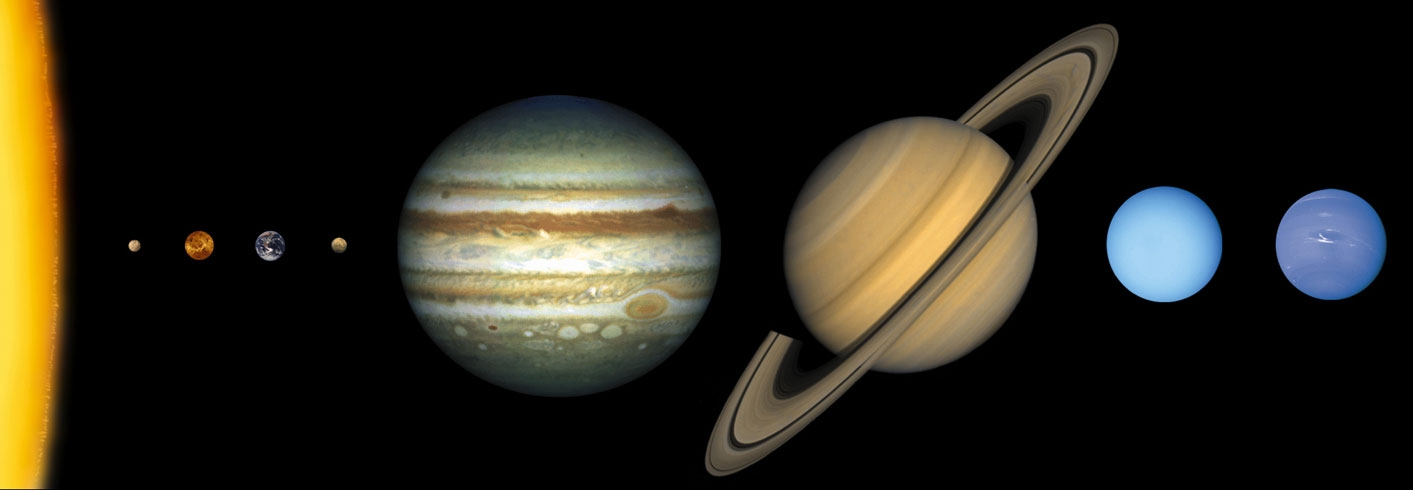
\includegraphics[width=0.9\textwidth{},keepaspectratio]{sun.jpg}
  \caption{太阳系}
  \label{fig:sun}
\end{figure}

\begin{table}[htbp]
  \caption{行星数据表1}
  \label{tab:xingxing}
  \centering
  \vspace{0.2cm}
  \wuhao
  \begin{tabular}{cccc}
    \toprule
    Planet  & Size(Earth=1) & Weight(Earth=1) & Radius  \\
    \midrule
    Mercury & 0.056         & 0.055           & 0.3871  \\
    Venus   & 0.857         & 0.815           & 0.7233  \\
    Earth   & 1.00          & 1.000           & 1.0000  \\
    Mars    & 0.151         & 0.107           & 1.5237  \\
    Jupiter & 1321          & 317.832         & 5.2026  \\
    Saturn  & 755           & 95.16           & 9.5549  \\
    Uranus  & 63            & 14.54           & 19.2184 \\
    Neptune & 58            & 17.15           & 30.1104 \\
    \bottomrule
  \end{tabular}
\end{table}

表~\ref{tab:xingxing}的源代码如下:
\vspace{1em}
\begin{lstlisting}
  \begin{table}[htbp]
    \caption{行星数据表1}
    \label{tab:xingxing}
    \centering
    \vspace{0.2cm}
    \wuhao
    \begin{tabular}{cccc}
      \toprule
      Planet  & Size(Earth=1) & Weight(Earth=1) & Radius  \\
      \midrule
      Mercury & 0.056         & 0.055           & 0.3871  \\
      Venus   & 0.857         & 0.815           & 0.7233  \\
      Earth   & 1.00          & 1.000           & 1.0000  \\
      Mars    & 0.151         & 0.107           & 1.5237  \\
      Jupiter & 1321          & 317.832         & 5.2026  \\
      Saturn  & 755           & 95.16           & 9.5549  \\
      Uranus  & 63            & 14.54           & 19.2184 \\
      Neptune & 58            & 17.15           & 30.1104 \\
      \bottomrule
    \end{tabular}
  \end{table}
\end{lstlisting}

表格和插图通常需要占据大块空间,所以在文字处理软件中用户经常需要调整它们的
位置。 \texttt{table}环境可以自动完成这样的任务,这种自动调整位置的环境称作
浮动环境 (float)\footnote{下一节里还会介绍插图浮动环境}。table环境是一个将表格嵌入文本的浮动环境。

\texttt{htbp} 选项用来指定表格的理想位置,这几个字母分别代表 here, top,
bottom,float page,也就是就这里、页顶、页尾、浮动页 (专门放浮动环境的单独
页面)。我们可以使用这几个字母的任意组合,四个字母都写上表示放哪里都无所
谓;一般不推荐单独使用\texttt{h},因为 \LaTeX{}自以为它的排版算法是最完美的,不愿意
被束缚手脚。

\verb|\centering| 用来使表格居
中; \verb|\caption| 命令设置表格标题, \LaTeX{}会自动给
浮动环境的标题加上编号。

它的官方使用说明为:
\begin{lstlisting}
  \caption{ 标题 }
  \label{label}
\end{lstlisting}
可选参数~label~用来作为交叉引用链接。例如
表~\ref{tab:xingxing}中的 lable为 tab:xingxing 。这里的标
签一般为英文。中文短标题一般没什么用,可以随意填。最简单就是“表”。

在表格环境中,标题必须位于表格的上方。而在图片环境中,标题的位置必须位于
图片的下方。

tabular 环境提供了最简单的表格功能。它用 \texttt{\&} 来分列,
用 \texttt{\textbackslash{\textbackslash{}}} 来换行;每列可以采用居中、居
左、居右等横向对齐方式,分别用 \texttt{l、c、r} 来表示。

三线表的三条横线就分别
用 \verb|\toprule、 \midrul、\bottomrule| 等命令表示。

\verb|\vspace{0.2cm}| 是用来控制表格标题与表格正文的
垂直间距的,请在插入表格时务必添加。 \verb|\wuhao| 是
用来调整表格内容的行距的。


\subsection{多列三线表}

在三线表中,有些列的列头会横跨好几列的数据。一般使
用 \verb|\multicolumn| 命令。它的用法是:
\begin{lstlisting}
  \multicolumn{ 列数}{ 对齐方式 }{ 表格内容 }
\end{lstlisting}

“列数”是指这一列横跨的列数,在表~\ref{tab:linux}是2列,就填“2”;“对
齐方式”从\texttt{lcr}三者中选其一即可,在表~\ref{tab:linux}中是\texttt{c}。“表格
内容”填入自己的内容。一般还会在这一列的下面画一小横线,已示辨识。使
用 \verb|\cmidrule| 命令。在表~\ref{tab:linux}中,由于横跨的是第2列和第3列,
因此 \verb|\cmidrule| 的参数是2-3。

\begin{table}[htbp]
  \caption{不同操作系统下的\LaTeX{}}
  \label{tab:linux}
  \centering
  \vspace{0.2cm}
  \wuhao
  \begin{tabular}{ccc}
    \toprule
    Test       & \multicolumn{2}{c}{Common Tools}             \\
    \cmidrule{2-3}
    OS         & Distribution                     & Editor    \\
    \midrule
    Windows    & MikTeX                           & TexMakerX \\
    Mac OS     & MacTeX                           & TeXShop   \\
    Linux/Unix & TeX Live                         & TeXworks  \\
    \bottomrule
  \end{tabular}
\end{table}


\begin{lstlisting}
  \begin{table}[htbp]
    \caption{不同操作系统下的\LaTeX{}}
    \label{tab:linux}
    \centering
    \vspace{0.2cm}
    \wuhao
    \begin{tabular}{ccc}
      \toprule
      Test    & \multicolumn{2}{c}{Common Tools} \\
                \cmidrule{2-3}
      OS         & Distribution & Editor  \\
      \midrule
      Windows    & MikTeX       & TexMakerX  \\
      Mac OS     & MacTeX       & TeXShop  \\
      Linux/Unix & TeX Live     & TeXworks  \\
      \bottomrule
    \end{tabular}
  \end{table}
\end{lstlisting}

\subsection{多行三线表}

既然有多列三线表,多行三线表也是用类似的方法解决。我们把表~\ref{tab:linux} 来改造一下,相对应的,一般使用 \verb|\multirow| 命令。它的用法
是:
\begin{lstlisting}
  \multirow{ 行数 }*{ 表格内容 }
\end{lstlisting}

“行数”是指竖向跨的行数,在表~\ref{tab:unix}中是2行,中间有个星号,表示自然宽度。

\begin{table}[htbp]
  \caption{不同操作系统下的\LaTeX{}}
  \label{tab:unix}
  \centering
  \vspace{0.2cm}
  \wuhao
  \begin{tabular}{ccc}
    \toprule
    \multirow{2}*{OS} & \multicolumn{2}{c}{Common Tools}             \\
    \cmidrule{2-3}
                      & Distribution                     & Editor    \\
    \midrule
    Windows           & MikTeX                           & TexMakerX \\
    Mac OS            & MacTeX                           & TeXShop   \\
    Linux/Unix        & TeX Live                         & TeXworks  \\
    \bottomrule
  \end{tabular}
\end{table}


\begin{lstlisting}
  \begin{table}[htbp]
    \caption{不同操作系统下的\LaTeX{}}
    \label{tab:unix}
    \centering
    \vspace{0.2cm}
    \wuhao
    \begin{tabular}{ccc}
      \toprule
      \multirow{2}*{OS} & \multicolumn{2}{c}{Common Tools} \\
                          \cmidrule{2-3}
                        & Distribution & Editor  \\
      \midrule
      Windows          & MikTeX       & TexMakerX  \\
      Mac OS           & MacTeX       & TeXShop  \\
      Linux/Unix       & TeX Live     & TeXworks  \\
      \bottomrule
    \end{tabular}
  \end{table}
\end{lstlisting}

\section{列宽可调表格的绘制方法}

论文中能用到列宽可调表格的情况共有两种,一种是当插入的表格某一单元格内容过长以至于一行放不下的情况,
另一种是当对公式中首次出现的物理量符号进行注释的情况,这两种情况都需要调用~tabularx~宏包。下面将分别对这两种情况下可调表格的绘制方法进行阐述。

\subsection{宽度控制}[Width Setting]

有时候表格中的某行太长了,需要折行。可以使用\texttt{tabularx} 宏包的同名
环境,其语法如下:

\begin{lstlisting}
  \begin{tabularx}{ 表格总宽度 }{ 对齐方式 }
    ...
  \end{tabularx}
\end{lstlisting}

“表格总宽度”最好用\texttt{textwidth}乘以某个系数表示。例
如\texttt{0.8\textbackslash{textwidth}}表示表格宽度是版芯宽度的0.8倍。这
样出来的效果比较好看。对齐方式除了原有的\texttt{l,c,r}之外,多了一
个\texttt{X},表示某列可以折行。

\begin{table}[htbp]
  \centering
  \caption{墙上的44句话}
  \label{tab:wall44}
  \vspace{0.2cm}
  \wuhao
  \begin{tabularx}{0.8\textwidth{}}{lX}
    \toprule
    People        & Says                                                 \\
    \midrule
    Elias Canetti & If you were alone, you would cut yourself in two, so
    that one part would shape the other.                                 \\
    Franz Kafka   & In the struggle between yourself and the world,
    second the world.                                                    \\
    \bottomrule
  \end{tabularx}
\end{table}

\begin{lstlisting}
  \begin{table}[htbp]
    \centering
    \caption{墙上的44句话}
    \label{tab:wall44}
    \vspace{0.2cm}
    \wuhao
    \begin{tabularx}{0.8\textwidth{}}{lX}
      \toprule
      People & Says \\
      \midrule Elias Canetti & If you were alone, you would cut yourself
      in two, so  that one part would shape the other.\\
      Franz Kafka & In the struggle between yourself and the world,
      second the world.\\
      \bottomrule
    \end{tabularx}
  \end{table}
\end{lstlisting}

\subsection{表格内某单元格内容过长的情况}

首先给出这种情况下的一个例子如表~\ref{table3}~所示。
\begin{table}[htbp]
  \centering
  \caption{最小的三个正整数的英文表示法}
  \label{table3}
  \vspace{0.5em}\wuhao
  \begin{tabularx}{0.7\textwidth}{llX}
    \toprule[1.5pt]
    Value & Name  & Alternate names, and names for sets of the given size                                                                                           \\\midrule[1pt]
    1     & One   & ace, single, singleton, unary, unit, unity                                                                                                      \\
    2     & Two   & binary, brace, couple, couplet, distich, deuce, double, doubleton, duad, duality, duet, duo, dyad, pair, snake eyes, span, twain, twosome, yoke \\
    3     & Three & deuce-ace, leash, set, tercet, ternary, ternion, terzetto, threesome, tierce, trey, triad, trine, trinity, trio, triplet, troika, hat-trick     \\\bottomrule[1.5pt]
  \end{tabularx}
\end{table}

绘制这种表格的代码及其说明如下。
\vspace{1em}
\begin{lstlisting}
\begin{table}[htbp]
\caption{标题}
\label{标签名}
\vspace{0.5em}\wuhao
\begin{tabularx}{\textwidth}{l...X...l}
\toprule[1.5pt]
表头第1个格   & ... & 表头第X个格   & ... & 表头第n个格  \\
\midrule[1pt]
表中数据(1,1) & ... & 表中数据(1,X) & ... & 表中数据(1,n)\\
表中数据(2,1) & ... & 表中数据(2,X) & ... & 表中数据(2,n)\\
.........................................................\\
表中数据(m,1) & ... & 表中数据(m,X) & ... & 表中数据(m,n)\\
\bottomrule[1.5pt]
\end{tabularx}
\end{table}
\end{lstlisting}


tabularx环境共有两个必选参数:第1个参数用来确定表格的总宽度,这里取为排版表格能达到的最大宽度——正文宽度 \verb|\textwidth| ;第2个参数用来确定每列格式,其中标为X的项表示该列的宽度可调,其宽度值由表格总宽度确定。
标为X的列一般选为单元格内容过长而无法置于一行的列,这样使得该列内容能够根据表格总宽度自动分行。若列格式中存在不止一个X项,则这些标为X的列的列宽相同,因此,一般不将内容较短的列设为X。
标为X的列均为左对齐,因此其余列一般选为\texttt{l}(左对齐),这样可使得表格美观,但也可以选为\texttt{c}或\texttt{r}。


\section{斜线表头}

还是有些童鞋的表示三线表不实用啊,非要回归到原来的斜线表头去。我们可以使
用宏包 diagbox 提供的命令轻松完成。不过呢,出来的表格很 ugly 罢了。

diagbox 是宏包提供的主要命令。它可以带有两个必选参数,表示要生成斜
线表头的两部分内容。默认斜线是从西北到东南方向的。

需要注意的是,使用斜线表格后就不能使用三线表的三条横线,不然请看
表~\ref{tab:diagbox}的下场。正确的做法是使用最原始的 hline,见
表~\ref{tab:xiexian}。

\begin{table}[htbp]
  \caption{斜线表头}
  \label{tab:diagbox}
  \centering
  \vspace{0.2cm}
  \wuhao
  \begin{tabular}{|l|ccc|}
    \toprule
    \diagbox{Times}{Day} & Mon  & Tue  & Wed  \\
    \midrule
    Morning              & used & used &      \\
    Afternoon            &      & used & used \\
    \bottomrule
  \end{tabular}
\end{table}

\begin{lstlisting}
  \begin{table}[htbp]
    \caption{斜线表头}
    \label{tab:diagbox}
    \centering
    \vspace{0.2cm}
    \wuhao
    \begin{tabular}{|l|ccc|}
      \toprule
      \diagbox{Times}{Day} & Mon  & Tue  & Wed  \\
      \midrule
      Morning              & used & used &  \\
      Afternoon            &      & used & used \\
      \bottomrule
    \end{tabular}
  \end{table}
\end{lstlisting}

\begin{table}[htbp]
  \caption{斜线表头}
  \label{tab:xiexian}
  \centering
  \vspace{0.2cm}
  \wuhao
  \begin{tabular}{|l|ccc|}
    \hline
    \diagbox{Times}{Day} & Mon  & Tue  & Wed  \\
    \hline
    Morning              & used & used &      \\
    Afternoon            &      & used & used \\
    \hline
  \end{tabular}
\end{table}

\begin{lstlisting}
  \begin{table}[htbp]
    \caption{斜线表头}
    \label{tab:xiexian}
    \centering
    \vspace{0.2cm}
    \wuhao
    \begin{tabular}{|l|ccc|}
      \hline
      \diagbox{Times}{Day} & Mon  & Tue  & Wed  \\
      \hline
      Morning              & used & used &  \\
      Afternoon            &      & used & used \\
      \hline
    \end{tabular}
  \end{table}
\end{lstlisting}


\section{表格的列按小数点对齐}

以表~\ref{tab:xingxing}为例,想把其中的第三列按小数点对齐\footnote{参见宏
  包siunitx}。先看一下效果:

在表~\ref{tab:xiaoshu}中,我们调整了原来四列数的对齐方式。原来
是\texttt{cccc},现在是\texttt{lcSr}。第一列左对齐,第二列不变,还是居中
对齐,第四列右对齐。值得注意的是第三列,这里新引入了一个参数\texttt{S},
含义就是这一列的数字按照小数点对齐。一定是大写的\texttt{S}。另外,第三列的列
头Weight(Earth=1)两边也加上了大括号,因为这不是数字。在使用参
数\texttt{S}的时候,不是数字的行需要用大括号括起来,不然会造成编译错误。

\begin{table}[htbp]
  \caption{行星数据表2}
  \label{tab:xiaoshu}
  \centering
  \vspace{0.2cm}
  \wuhao
  \begin{tabular}{lcSr}
    \toprule
    Planet  & Size(Earth=1) & {Weight(Earth=1)} & Radius  \\
    \midrule
    Mercury & 0.056         & 0.055             & 0.3871  \\
    Venus   & 0.857         & 0.815             & 0.7233  \\
    Earth   & 1.00          & 1.000             & 1.0000  \\
    Mars    & 0.151         & 0.107             & 1.5237  \\
    Jupiter & 1321          & 317.832           & 5.2026  \\
    Saturn  & 755           & 95.16             & 9.5549  \\
    Uranus  & 63            & 14.54             & 19.2184 \\
    Neptune & 58            & 17.15             & 30.1104 \\
    \bottomrule
  \end{tabular}
\end{table}

\begin{lstlisting}
  \begin{table}[htbp]
    \caption{行星数据表2}
    \label{tab:xiaoshu}
    \centering
    \vspace{0.2cm}
    \wuhao
    \begin{tabular}{lcSr}
      \toprule
      Planet  & Size(Earth=1) & {Weight(Earth=1)} & Radius  \\
      \midrule
      Mercury & 0.056         & 0.055           & 0.3871  \\
      Venus   & 0.857         & 0.815           & 0.7233  \\
      Earth   & 1.00          & 1.000           & 1.0000  \\
      Mars    & 0.151         & 0.107           & 1.5237  \\
      Jupiter & 1321          & 317.832         & 5.2026  \\
      Saturn  & 755           & 95.16           & 9.5549  \\
      Uranus  & 63            & 14.54           & 19.2184 \\
      Neptune & 58            & 17.15           & 30.1104 \\
      \bottomrule
    \end{tabular}
  \end{table}
\end{lstlisting}

\section{对物理量符号进行注释的情况}

为使得对公式中物理量符号注释的转行与破折号“——”后第一个字对齐,此处最好采用表格环境。此表格无任何线条,左对齐,
且在破折号处对齐,一共有“式中”二字、物理量符号和注释三列,表格的总宽度可选为文本宽度,因此应该采用\verb|tabularx|环境。
由\verb|tabularx|环境生成的对公式中物理量符号进行注释的公式如式(\ref{eq:1})所示。

\begin{equation}\label{eq:1}
  \ddot{\boldsymbol{\rho}}-\frac{\mu}{R_{t}^{3}}\left(3\mathbf{R_{t}}\frac{\mathbf{R_{t}\rho}}{R_{t}^{2}}-\boldsymbol{\rho}\right)=\mathbf{a}
\end{equation}
\begin{tabularx}{\textwidth}{@{}l@{\quad}r@{——}X@{}}
  式中 & $\boldsymbol{\rho}$        & 追踪飞行器与目标飞行器之间的相对位置矢量; \\
       & $\boldsymbol{\ddot{\rho}}$ & 追踪飞行器与目标飞行器之间的相对加速度;   \\
       & $\mathbf{a}$               & 推力所产生的加速度;                       \\
       & $\mathbf{R_t}$             & 目标飞行器在惯性坐标系中的位置矢量;       \\
       & $\omega_{t}$               & 目标飞行器的轨道角速度;                   \\
       & $\mathbf{g}$               & 重力加速度,$=\frac{\mu}{R_{t}^{3}}\left(
    3\mathbf{R_{t}}\frac{\mathbf{R_{t}\rho}}{R_{t}^{2}}-\boldsymbol{\rho}\right)=\omega_{t}^{2}\frac{R_{t}}{p}\left(
    3\mathbf{R_{t}}\frac{\mathbf{R_{t}\rho}}{R_{t}^{2}}-\boldsymbol{\rho}\right)$,这里~$p$~是目标飞行器的轨道半通径。
\end{tabularx}
\vspace{2em}

其中生成注释部分的代码及其说明如下。
\vspace{1em}
\begin{lstlisting}
\begin{tabularx}{\textwidth}{@{}l@{\quad}r@{— —}X@{}}
式中 & symbol-1 & symbol-1的注释内容;\\
     & symbol-2 & symbol-2的注释内容;\\
     .............................;\\
     & symbol-m & symbol-m的注释内容。
\end{tabularx}\vspace{2em}
\end{lstlisting}


tabularx环境的第1个参数~\verb|{\textwidth}|~设置表格宽度为正文宽度,第2个参数里面各个符号的意义为:
第1个~\verb|@{}l|~表示在“式中”二字左侧不插入任何文本,“式中”二字能够在正文中左对齐,若无此项,则“式中”二字左侧会留出一定的空白;
~\verb|@{\quad}|~表示在“式中”和物理量符号间插入一个空铅宽度的空白;
~\verb|@{— — }|~实现插入破折号的功能,它由两个个1/2的中文破折号构成;
第2个~\verb|@{}|~表示在注释内容靠近正文右边界的地方能够实现右对齐。


由此方法生成的注释内容应紧邻待注释公式并置于其下方,因此不能将代码放入\verb|table|浮动环境中。
但此方法不能实现自动转页接排,可能会在当前页剩余空间不够时,全部移动到下一页而导致当前页出现很大空白。
因此在需要转页处理时,需要手动将将原来的一个\verb|tabularx|环境拆分为两个\verb|tabularx|环境。

\subsubsection{排版横版表格的举例}
由于版面设置方向调整,使用横版排版的表格必须另起一页,例如表~\ref{table4}。

\begin{table}[p]
  \centering
  \begin{sideways}
    \begin{minipage}{\textheight}
      \caption{不在规范中规定的横版表格}
      \label{table4}
      \vspace{0.5em}\centering\wuhao
      \begin{tabular}{ccccc}
        \toprule[1.5pt]
        $D$(in) & $P_u$(lbs) & $u_u$(in) & $\beta$ & $G_f$(psi.in) \\
        \midrule[1pt]
        5       & 269.8      & 0.000674  & 1.79    & 0.04089       \\
        10      & 421.0      & 0.001035  & 3.59    & 0.04089       \\
        20      & 640.2      & 0.001565  & 7.18    & 0.04089       \\
        \bottomrule[1.5pt]
      \end{tabular}
    \end{minipage}
  \end{sideways}
\end{table}

\section{罗列}
学位论文一般可采用两种罗列环境:一种是并列条目有同样标签的~\verb|itemize|~罗列环境,
另一种是具有自动排序编号符号的~\verb|enumerate|~罗列环境。这两种罗列环境的样式参数可参考图~\ref{list}。
\begin{figure}[htbp]
  \centering
  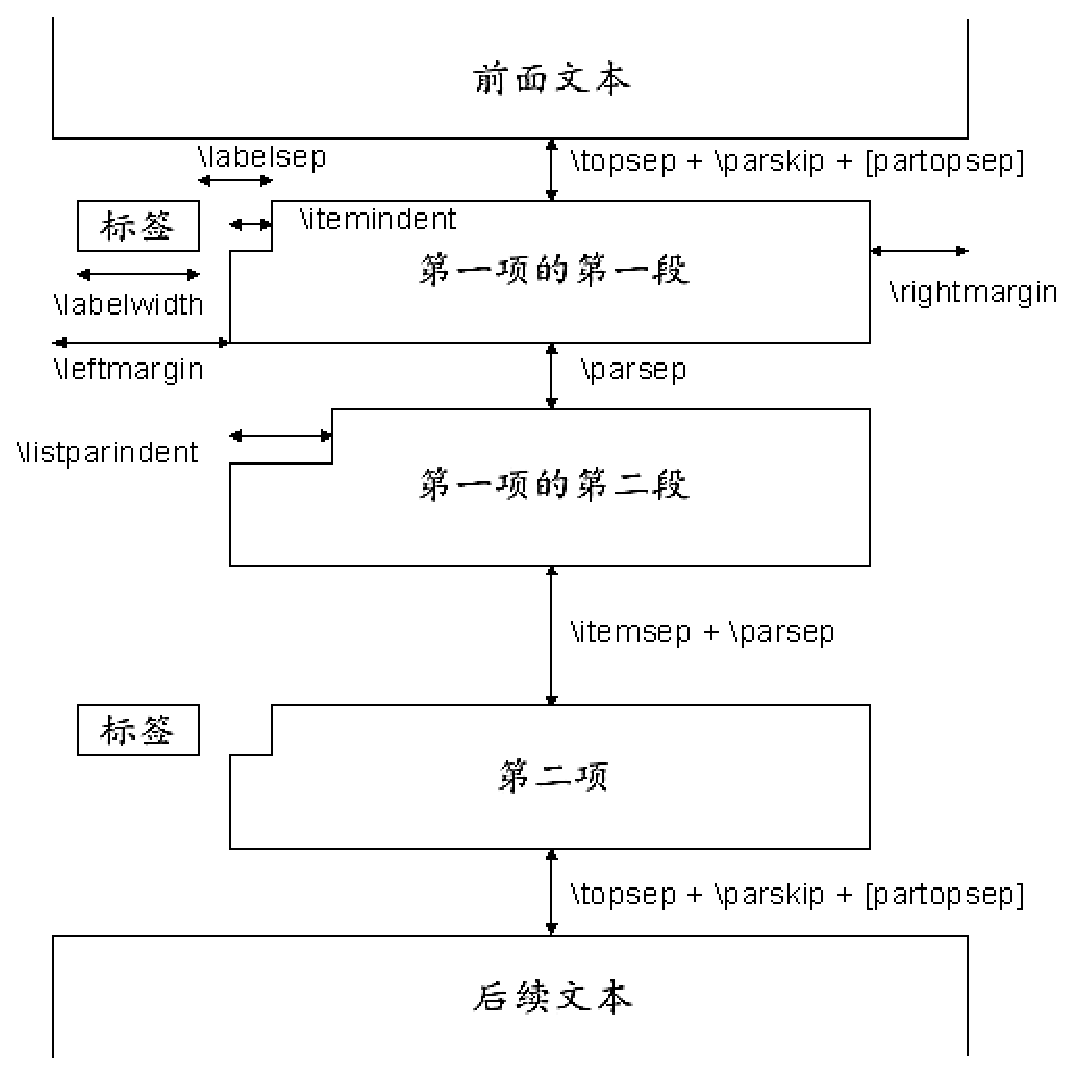
\includegraphics[width = 0.6\textwidth]{list}
  \caption{罗列环境参数示意图}
  \label{list}
  \vspace{-1em}
\end{figure}

通过调用~enumitem~宏包可以很方便地控制罗列环境的布局,
其~format.tex~文件中的~\verb|\setitemize|~和~\verb|\setenumerate|~命令分别用来设置~\verb|itemize|~和~\verb|enumerate|~环境的样式参数。
采用~\verb|itemize|~单层罗列环境的排版形式如下:

\begin{itemize}
  \item 第一个条目文本内容
  \item 第二个条目文本内容
  \item 第三个条目文本内容
\end{itemize}

其代码如下
\begin{verbatim}
\begin{itemize}
  \item 第一个条目文本内容
  \item 第二个条目文本内容
  ...
  \item 第三个条目文本内容
\end{itemize}
\end{verbatim}

采用~\verb|enumerate|~单层罗列环境的排版形式如下:
\begin{enumerate}
  \item 第一个条目文本内容
  \item 第二个条目文本内容
  \item 第三个条目文本内容
\end{enumerate}

其代码如下
\begin{verbatim}
\begin{enumerate}
  \item 第一个条目文本内容
  \item 第二个条目文本内容
  ...
  \item 第三个条目文本内容
\end{enumerate}
\end{verbatim}

例如:

\begin{enumerate}
  \item 鉴定袋蛾———二十分
  \item 给斯拉瓦写信———二小时四十五分
  \item 植物保护小组开会———二小时二十五分
\end{enumerate}

上述是默认的列表样式。源代码如下:
\begin{lstlisting}
  \begin{enumerate}
  \item 鉴定袋蛾———二十分
  \item 给斯拉瓦写信———二小时四十五分
  \item 植物保护小组开会———二小时二十五分
  \end{enumerate}
\end{lstlisting}

\texttt{emumerate}环境就是罗列环境。每条\verb|\item| 后面
跟一个空格,然后就是具体的罗列条目。

默认的样式是按照1.、2.、3.、……来排序的,如果想按照英文字母(a),(b),(c)或者罗
马数字(i),(ii),(iii)这样的顺序呢,只需要
在 \verb|\item[]| 后面[~]中加入指定的序号。比如:
\begin{enumerate}
  \item[(1)] 鉴定袋蛾———二十分
  \item[(2)] 给斯拉瓦写信———二小时四十五分
  \item[(3)] 植物保护小组开会———二小时二十五分
\end{enumerate}
源代码是:
\begin{lstlisting}
  \begin{enumerate}
  \item[(1)] 鉴定袋蛾———二十分
  \item[(2)] 给斯拉瓦写信———二小时四十五分
  \item[(3)] 植物保护小组开会———二小时二十五分
  \end{enumerate}
\end{lstlisting}

\section*{本章小结}
表格和罗列排版方法介绍。

%! TEX program = xelatex
%! TEX root = ../main.tex
%! TEX encoding = utf-8

%%%%%%%%%%%%%%%%%%%%%%%%%%%%%%%%%%%%%%%%%%%%%%%%%%%%%%%%%%%%%%%%%%%%%%
%
%  哈尔滨工程大学学位论文 XeLaTeX 模版 —— 正文文件 chap04.tex
%
%  版本:1.0.0
%  最后更新:
%  修改者:Leo LiWenhui lwh@hrbeu.edu.cn
%  修订者:
%  编译环境1:Ubuntu 12.04 + TeXLive 2013/2014
%  编译环境2:Windows 7/8  + TeXLive 2013/2014
%
%%%%%%%%%%%%%%%%%%%%%%%%%%%%%%%%%%%%%%%%%%%%%%%%%%%%%%%%%%%%%%%%%%%%%

\chapter{插图}[Figure]
\label{chap05}

\section{研究生院的插图规范}[Requirement of Figure]
图应有自明性。插图应与文字紧密配合,文图相符,内容正确。选图要力求精练,插图、照片应完整清晰。图中文字和数字等字号用宋体~5~号字。

机械工程图:采用第一角投影法,严格按照~GB4457---GB131-83《机械制图》标准规定。

数据流程图、程序流程图、系统流程图等按~GB1526-89~标准规定。

电气图:图形符号、文字符号等应符合附录~3~所列有关标准的规定。

流程图:必须采用结构化程序并正确运用流程框图。

对无规定符号的图形应采用该行业的常用画法。

坐标图的坐标线均用细实线,粗细不得超过图中曲线,有数字标注的坐标图,必须注明坐标单位。

照片图要求主题和主要显示部分的轮廓鲜明,便于制版。如用放大或缩小的复制品,必须清晰,反差适中。照片上应有表示目的物尺寸的标度。

引用文献图表必须标注出处。


\subsection{图题及图中说明}[Note of Figure]
每个图均应有图题(由图序和图名组成),图名在图序之后空一格排写。图序按章编排,如第~1~章第一个插图的图号为“图~1.1”等。
图题置于图下,硕士论文可只用中文书写,博士论文用中、英文两种文字居中书写,中文在上,要求中文用宋体~5~号字,英文用~Times New Roman 5~号字。有图注或其它说明时应置于图题之上。引用图应注明出处,在图题右上角加引用文献号。
图中若有分图时,分图题置于分图之下或图题之下,分图号用~(a)、(b)等表示。

图中各部分说明应采用中文(引用的外文图除外)或数字项号,各项文字说明置于图题之上(有分图题者,置于分图题之上)。

\subsection{插图编排}[Arrangment of Figure]

插图之前,文中必须有关于本插图的提示,如“见图~1.1”、“如图~1.1~所示”等。插图与其图题为一个整体,不得拆开排写于两页。
插图处的该页空白不够排写该图整体时,则可将其后文字部分提前排写,将图移到次页。

\section{LaTeX~中推荐使用的图片格式}[Figure Foramt]

论文使用的图片都放在figure文件夹中,图片可以是~EPS、JPG、PDF等格式。插图浮动环境是\texttt{figure},基本命
令是\texttt{includegraphics},而在图片环境中,标题的位置必须位于图片的下方。

\section{单张图片}[Single Figure]

单张图片示例如图\ref{fig:wedding}所示。插入方法为插入浮动图后,在图片位置插入所需图片。一般需要使用段落设置将图形设置为居中,在图形两边插入水平填充也可实现居中。\textbackslash bicaption设置图形引用标识及图形标题,其格式为:

\begin{lstlisting}
\bicaption[fig:refname]{中文索引图名称}{中文图名称}{Eng_Index}{English Caption}
\end{lstlisting}

 引用图形时,需在图题处插入“图\textbackslash ref~\{fig:refname\}”,\LaTeX{}编译器会自动对插图序号进行编排,并用最终图号替换符号引用标识。

 如果图形图题过长,\LaTeX{}排版系统会自动按悬挂缩进排版。

\begin{figure}[htbp]
  \centering
  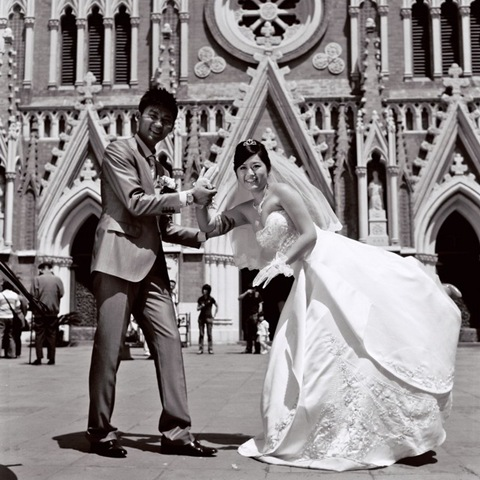
\includegraphics[scale=0.6]{wedding.jpg}
  \bicaption[fig:wedding]{婚礼}{婚礼}{Fig.}{Wedding}
\end{figure}

\begin{lstlisting}
  \begin{figure}[htbp]
    \centering
    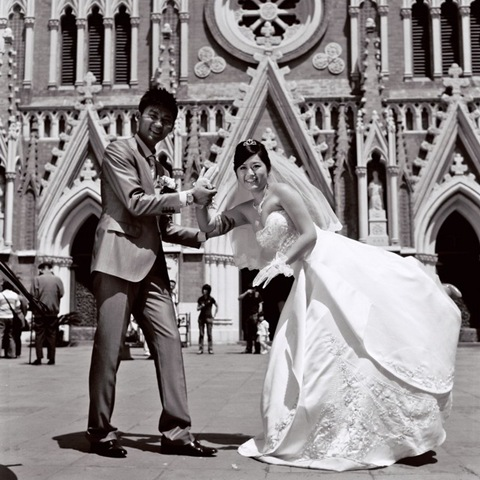
\includegraphics[scale=0.6]{wedding.jpg}
    \bicaption[fig:wedding]{婚礼}{婚礼}{Fig.}{Wedding}
  \end{figure}
\end{lstlisting}

\texttt{includegraphics}的基本参数见表~\ref{tab:figure}。

\begin{table}[htbp]
  \centering
  \bicaption[tab:figure]{插图命令参数}{插图命令参数}{Tab.}{Parameter}
  \vspace{0.2cm}
  \wuhao
  \begin{tabularx}{0.8\textwidth{}}{lX}
    \toprule
    参数             & 说明 \\
    \midrule
    width=x,height=y & 宽度和高度,绝对尺寸,可用任意长度单位。  \\
    scale=s          & 缩放比。绝对尺寸和缩放比用一种即可,同时使用两者,绝对尺寸起作用。 \\
    keepaspectratio & 保持图形比例。宽度和高度通常设置一个即可,否则图形比
    例会失调,除非再加上此选 项,
    这样图形宽度和高度都不超过指定参数。     \\
    angle=a          & 逆时针旋转角度,单位是度。  \\
    \bottomrule
  \end{tabularx}
\end{table}

对于图~\ref{fig:wedding},只使用了\texttt{scale}这一个参数,缩放因子是0.6。
当然,也可以直接指定图形的宽度和高度。图~\ref{fig:sun}的源代码如下:

\begin{lstlisting}
  \begin{figure}[htbp]
    \centering
    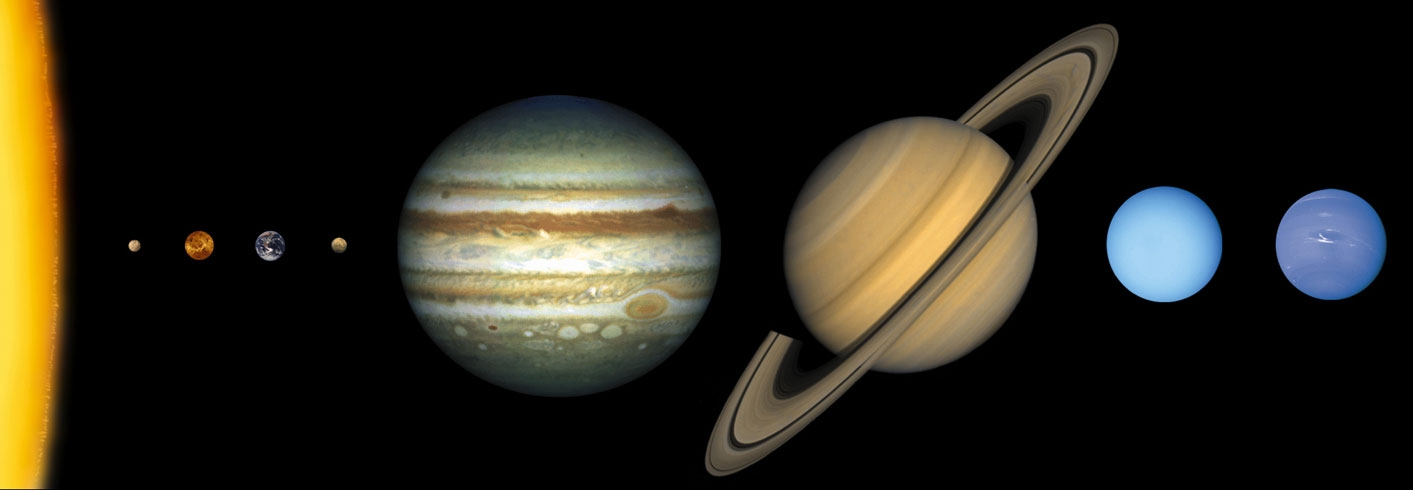
\includegraphics[width=\textwidth{},keepaspectratio]{sun.jpg}
    \bicaption[fig:sun]{太阳系}{最左侧是太阳,向右依序为水星、金
      星}{Fig.}{Outward from the Sun, the planets are Mercury, Venus,
      Earth, Mars, Jupiter, Saturn, Uranus and Neptune.}
  \end{figure}
\end{lstlisting}

可以看到,图~\ref{fig:sun}的宽度指定为版芯的宽度,然后使用了保持宽高比这
个选项。

\begin{figure}[tbph]
\usetikzlibrary{calc,through}
  \centering
    \begin{tikzpicture}
    \coordinate [label=left:$A$] (A) at (0,0);
    \coordinate [label=right:$B$] (B) at (0.75,0.25);
    \coordinate [label=above:$C$] (C) at (1,1.5);
    \draw (A) -- (B) -- (C);
    \coordinate [label=above:$D$] (D) at
    ($ (A) ! .5 ! (B) ! {sin(60)*2} ! 90:(B) $) {};
    \node (H) [label=135:$H$,draw,circle through=(C)] at (B) {};
    \draw (D) -- ($ (D) ! 3.5 ! (B) $) coordinate [label=below:$F$] (F);
    \draw (D) -- ($ (D) ! 2.5 ! (A) $) coordinate [label=below:$E$] (E);
    \end{tikzpicture}

    \bicaption[fig:sun]
    {长标题示例}
    {一个很长很长很长很长很长很长很长很长很长很长很长很长很长很长很长的标题示例
    这个图形是由Tikz绘制当然你也可以用JPG图片}
    {Fig.}
    {a long long long long long long long long long long long long caption}
\end{figure}

\begin{lstlisting}
    \begin{figure}[tbph]
        \usetikzlibrary{calc,through}
        \centering
        \begin{tikzpicture}
            \coordinate [label=left:$A$] (A) at (0,0);
            \coordinate [label=right:$B$] (B) at (0.75,0.25);
            \coordinate [label=above:$C$] (C) at (1,1.5);
            \draw (A) -- (B) -- (C);
            \coordinate [label=above:$D$] (D) at
            ($ (A) ! .5 ! (B) ! {sin(60)*2} ! 90:(B) $) {};
            \node (H) [label=135:$H$,draw,circle through=(C)] at (B) {};
            \draw (D) -- ($ (D) ! 3.5 ! (B) $) coordinate [label=below:$F$] (F);
            \draw (D) -- ($ (D) ! 2.5 ! (A) $) coordinate [label=below:$E$] (E);
        \end{tikzpicture}

        \bicaption[fig:sun]
        {长标题示例}
        {一个很长很长很长很长很长很长很长很长很长很长很长很长很长很长很长
        的标题示例这个图形是由TikZ绘制当然你也可以用JPG图片}
        {Fig.}
        {a long long long long long long long long long long long long caption}
    \end{figure}
\end{lstlisting}

长图题一般没有必要在插图目录中也完整显示,可使用菜单\texttt{Insert -{}-\textgreater{} Short
Title} 插入短标题 \verb|\index{ct\@插图\!dbt\@ 短标题} |。模板中已将图表编号两边设置了小的间距,不必再手动加入空格。


\section{双图并列}[Two Figures]

并列图示例如图\ref{fig:lang}与图\ref{fig:niang}所示。

\begin{figure}[htbp]
  \centering
  \begin{minipage}{0.4\textwidth}
    \centering
    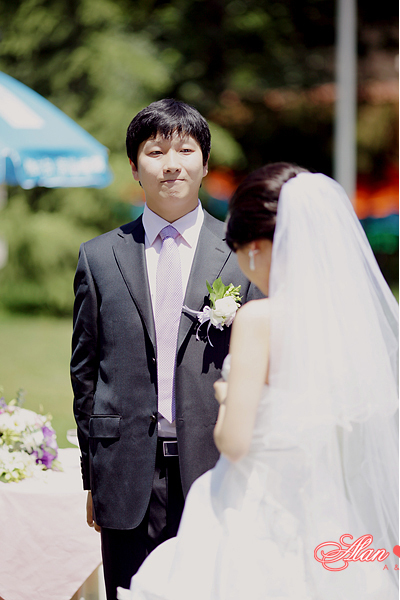
\includegraphics[keepaspectratio]{lang.jpg}
    \bicaption[fig:lang]{新郎}{新郎}{Fig.}{Bridegroom}
  \end{minipage}
  \begin{minipage}{0.4\textwidth}
    \centering
    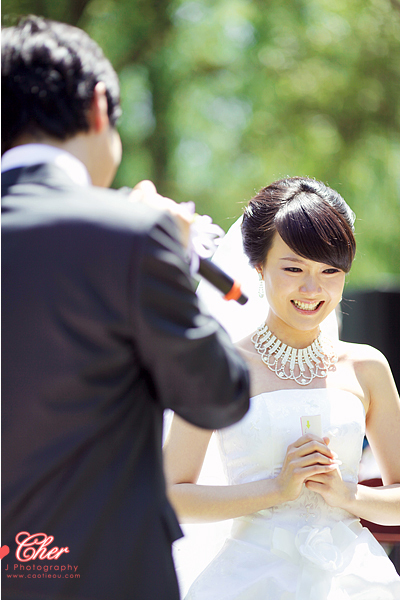
\includegraphics[keepaspectratio]{niang.jpg}
    \bicaption[fig:niang]{新娘}{新娘}{Fig.}{Brige}
  \end{minipage}
\end{figure}

\begin{lstlisting}
  \begin{figure}[htbp]
    \centering
    \begin{minipage}{0.4\textwidth}
      \centering
      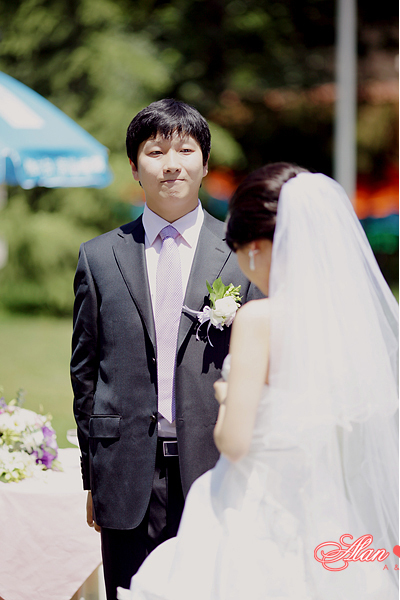
\includegraphics[keepaspectratio]{lang.jpg}
      \bicaption[fig:lang]{新郎}{新郎}{Fig.}{Bridegroom}
    \end{minipage}
    \begin{minipage}{0.4\textwidth}
      \centering
      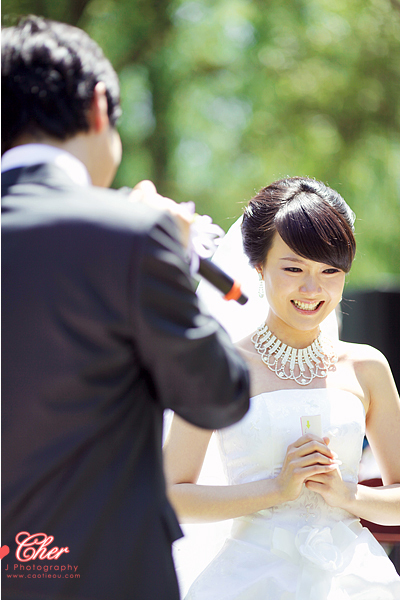
\includegraphics[keepaspectratio]{niang.jpg}
      \bicaption[fig:niang]{新娘}{新娘}{Fig.}{Brige}
    \end{minipage}
  \end{figure}
\end{lstlisting}

如果想要两幅并排的插图各有自己的标题,可以在 figure 环境中使用两
个 minipage 环境,每个里面插入一幅图 (见图~\ref{fig:lang}和
图~\ref{fig:niang}) 。不用 minipage 的话,因为插图标题的缺省宽度是
整个行宽,两幅插图就会上下排列。

这里指定了每个 minipage 的宽度为0.4倍的版芯宽度。当然,也可以自
己指定,只是两个宽度加起来不超过版芯宽度就可以了。

\section{两子图并列}[Sub Figure]

子图并列示例如图\ref{fig:judy}所示。

\begin{figure}[htbp]
    \centering
    \subfigure{\label{{fig:1a}}}\addtocounter{subfigure}{-2}
    \subfigure[Girl A]{\subfigure[女孩A]{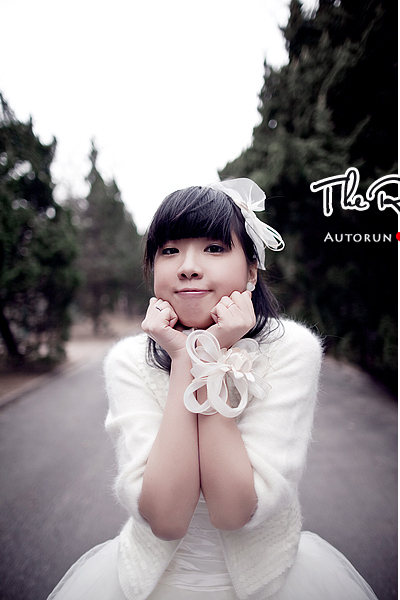
\includegraphics[keepaspectratio]{chao.jpg}}}
    \hspace{20pt}
    \subfigure{\label{{fig:1b}}}\addtocounter{subfigure}{-2}
    \subfigure[Girl B]{\subfigure[女孩B]{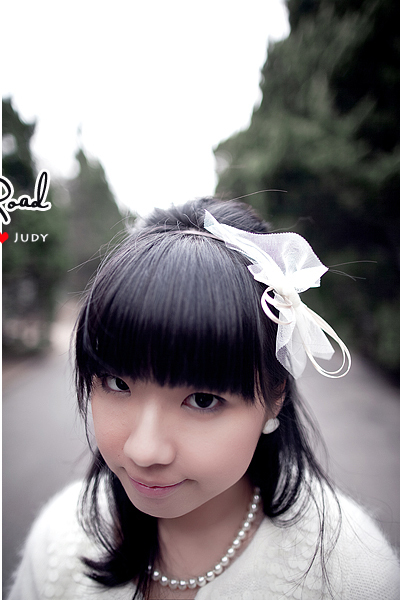
\includegraphics[keepaspectratio]{ren.jpg}}}
    \bicaption[fig:judy]{女孩}{女孩}{Fig.}{Judy}
\end{figure}

\begin{lstlisting}
  \begin{figure}[htbp]
    \centering
    \subfigure{\label{{fig:1a}}}\addtocounter{subfigure}{-2}
    \subfigure[Girl A]{\subfigure[女孩A]{
        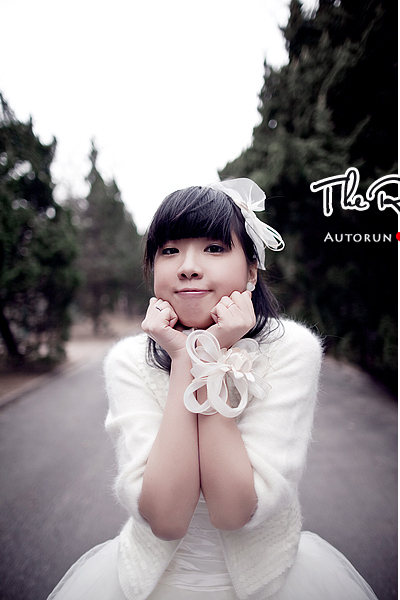
\includegraphics[keepaspectratio]{chao.jpg}}
    }
    \hspace{20pt}
    \subfigure{\label{{fig:1b}}}\addtocounter{subfigure}{-2}
    \subfigure[Girl B]{\subfigure[女孩B]{
        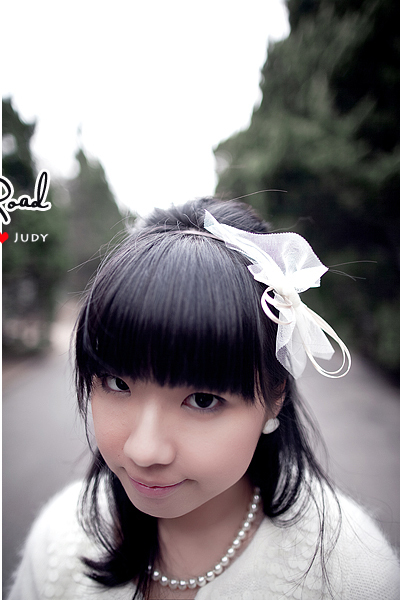
\includegraphics[keepaspectratio]{ren.jpg}}
    }
    \bicaption[fig:judy]{女孩}{女孩}{Fig.}{Judy}
  \end{figure}
\end{lstlisting}


如果想要两幅并排的图片共享一个标题,并且各有自己的子标题,学位论文规范要求不止总图的标题为中英文形式,其各个子图也应具有中英文形式的标题。
然而~ccaption~宏包却无法实现子图的中英文标题功能,这里采用对 \verb|\subfigure| 命令进行嵌套的方法来实现子图的中英文标题功能。如图~\ref{fig:judy},子图的标题用命令 \verb|\subcaption| 即可。
学位论文规范要求不止总图的标题为中英文形式,其各个子图也应具有中英文形式的标题。
然而~ccaption~宏包却无法实现子图的中英文标题功能,这里采用对 \verb|\subfigure| 命令进行嵌套的方法来实现子图的中英文标题功能。


\section{pgf/TikZ~插图}[pgf/TikZ Figure]
pgf/TikZ是一个在tex系统中的画图宏包,除了可以精确的作图外,对于某些不要求精确控制的图形绘制,如:流程图,树图,等等,也提供了简便易用的支持。
下面这张图片是用TikZ宏包进行绘制的图形,其实现代码为:
\begin{lstlisting}
    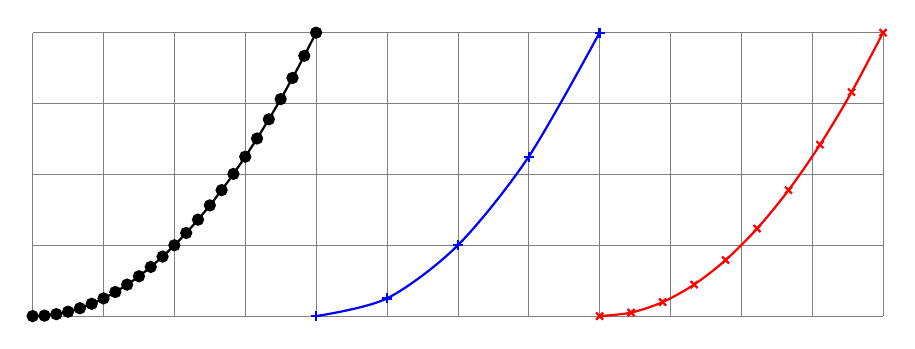
\begin{tikzpicture}[thick,smooth,domain=0:4,scale=0.9]
        \draw[very thin,gray] (0,0) grid (12,4);
        \draw plot[mark=*] (\x,{\x * \x/4});
        \draw[blue,xshift=4cm] plot[samples=5,mark=+] (\x,{\x * \x/4});
        \draw[red,xshift=8cm] plot[samples=10,mark=x] (\x,{\x * \x/4});
    \end{tikzpicture}
\end{lstlisting}

\begin{figure}[htbp]
    \centering
    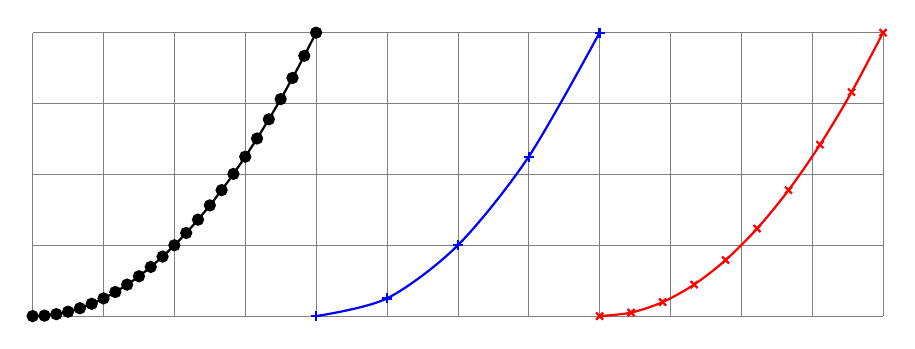
\begin{tikzpicture}[thick,smooth,domain=0:4,scale=0.9]
        \draw[very thin,gray] (0,0) grid (12,4);
        \draw plot[mark=*] (\x,{\x * \x/4});
        \draw[blue,xshift=4cm] plot[samples=5,mark=+] (\x,{\x * \x/4});
        \draw[red,xshift=8cm] plot[samples=10,mark=x] (\x,{\x * \x/4});
    \end{tikzpicture}
  \bicaption[fig:TikZ]{TikZ插图}{TikZ插图}{Fig.}{Draw with TikZ}
\end{figure}

更多的关于pgf/TikZ请参考相关资料。

\section*{本章小结}[Brief Summary]
插图方法介绍。

%! TEX program = xelatex
%! TEX root = ../main.tex
%! TEX encoding = utf-8

%%%%%%%%%%%%%%%%%%%%%%%%%%%%%%%%%%%%%%%%%%%%%%%%%%%%%%%%%%%%%%%%%%%%%%
%
%  哈尔滨工程大学学位论文 XeLaTeX 模版 —— 正文文件 chap04.tex
%
%  版本:1.0.0
%  最后更新:
%  修改者:Leo LiWenhui lwh@hrbeu.edu.cn
%  修订者:
%  编译环境1:Ubuntu 12.04 + TeXLive 2013/2014
%  编译环境2:Windows 7/8  + TeXLive 2013/2014
%
%%%%%%%%%%%%%%%%%%%%%%%%%%%%%%%%%%%%%%%%%%%%%%%%%%%%%%%%%%%%%%%%%%%%%

\chapter{数学公式的排版}
\label{chap06}

\section{公式规范}

论文中的公式应另起行,原则上应居中书写,与周围文字留有足够的空间区分开。
若公式前有文字(如“解”、“假定”等),文字空两格写,公式仍居中写。公式末不加标点。

公式应标注序号,并将序号置于括号内。 公式序号按章编排,如第~1~章第一个公式序号为“(1.1)”。公式的序号右端对齐。

公式较长时最好在等号“=”处转行,如难实现,则可在~$+$、$-$、$\times$、$\div$~运算符号处转行,转行时运算符号仅书写于转行式前,不重复书写。

文中引用公式时,一般用“见式~(1.1)”或“由公式~(1.1)”。

公式中用斜线表示“除”的关系时应采用括号,以免含糊不清,如~$a/(b\cos x)$。通常“乘”的关系在前,如~$a\cos x/b$而不写成~$(a/b)\cos x$。

不能用文字形式表示等式,如:$\textnormal{刚度}=\frac{{\textnormal{受力}}}{{\textnormal{受力方向的位移}}}$。

\textbf{对于数学公式的输入方法,网络上有一个比较全面权威的文档~\href{http://tug.ctan.org/cgi-bin/ctanPackageInformation.py?id=voss-mathmode}{Math mode}~请大家事先大概浏览一下。下面将对学位论文中主要用到的数学公式排版形式进行阐述。}

\section{生成~LaTeX~数学公式的两种方法}[Methods of Equation]

对于先前没有接触过~\LaTeX~的人来说,编写~\LaTeX~数学公式是一件很繁琐的事,尤其是对复杂的数学公式来说,更可以说是一件难以完成的任务。
实际上,生成~\LaTeX~数学公式有一种基于~MathType~数学公式编辑器的简便方法。

MathType~是一款功能强大的数学公式编辑器软件,能够用来在文本环境中插入~Windows OLE~图形格式的复杂数学公式,所以应用比较普遍。但此软件只有~30~天的试用期,之后若再继续使用则需要付费购买才行。网络上有很多破解版的~MathType~软件可供下载免费使用,
笔者推荐下载安装版本号在~6.5~之上的中文破解版。

在安装好~MathType~之后,若在输入窗口中编写数学公式,复制到剪贴板上的仍然是图形格式的对象。
若希望得到可插入到~\LaTeX~编辑器中的文本格式对象,则需要对~MathType~软件做一下简单的设置:在~MathType~最上排的按钮中依次选择“参数选项
$\to$转换”,在弹出的对话窗中选中“转换到其它语言(文字):”,在转换下拉框中选择“Tex~--~--~LaTeX 2.09 and later”,并将对话框最下方的两个复选框全部勾掉,点击确定,这样,再从输入窗口中复制出来的对象就是文本格式的了,就可以直接将其粘贴到~\LaTeX~
编辑器中了。按照这种方法生成的数学公式两端分别有标记\verb|\[|和标记\verb|\]|,在这两个标记之间才是真正的数学公式代码。

若希望从~MathType~输入窗口中复制出来的对象为图形格式,则只需再选中“公示对象(Windows OLE~图形)”即可。


\section{行内公式}

出现在正文一行之内的公式称为行内公式,例如~$f(x)=\int_{a}^{b}\frac{\sin{x}}{x}\mathrm{d}x$。对于非矩阵和非多行形式的行内公式,一般不会使得行距发生变化,而~word~等软件却会根据行内公式的竖直距离而自动调节行距,如图~\ref{hangju}~所示。
\begin{figure}[htbp]
  \centering
  \subfigure{\label{latex}}\addtocounter{subfigure}{-2}
  \subfigure[Inline mode equation derived from \LaTeX system]{\subfigure[由~\LaTeX~系统生成的行内公式]
    {\fbox{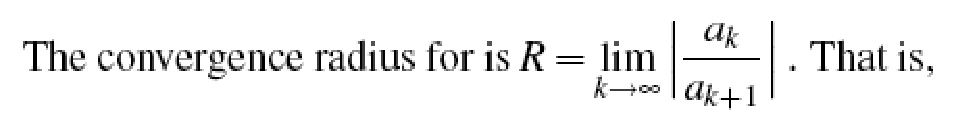
\includegraphics[width=0.55\textwidth]{latex}}}}
  \subfigure{\label{word}}\addtocounter{subfigure}{-2}
  \subfigure[Inline mode equation displayed as .doc format file derived from word software]{\subfigure[由~word软件生成的~.doc~格式行内公式]
    {\fbox{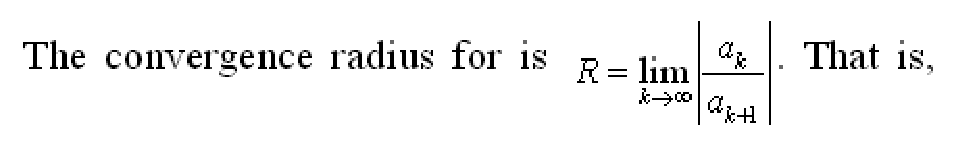
\includegraphics[width=0.55\textwidth]{word}}}}
  \subfigure{\label{pdf}}\addtocounter{subfigure}{-2}
  \subfigure[Inline mode equation displayed as .pdf format file derived from word software]{\subfigure[由~word软件生成的~.pdf~格式行内公式]
    {\fbox{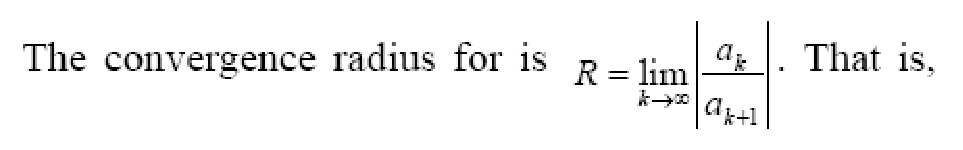
\includegraphics[width=0.55\textwidth]{pdf}}}}
  \caption{由~\LaTeX~和~word~生成的~3~种行内公式屏显效果}
  \label{hangju}
  \vspace{-1em}
\end{figure}
这三幅图分别为~\LaTeX~和~word~生成的行内公式屏显效果,从图中可看出,在~\LaTeX~文本含有公式的行内,在正文与公式之间对接工整,行距不变;而在~word~文本含有公式的行内,在正文与公式之间对接不齐,行距变大。因此从这一点来说,
\LaTeX~系统在数学公式的排版上具有很大优势。

\LaTeX~提供的行内公式最简单、最有效的方法是采用~\TeX~本来的标记——开始和结束标记都写作~\$,例如本节开始的例子可由下面的输入得到。
\begin{lstlisting}
  $f(x)=\int_{a}^{b}\frac{\sin{x}}{x}\mathrm{d}x$
\end{lstlisting}

\section{行间公式}

位于两行之间的公式称为行间公式,每个公式都是一个单独的段落,例如
\[\int_a^b{f\left(x\right)\mathrm{d}x}=\lim_{\left\|\Delta{x_i}\right\|\to 0}\sum_i{f\left(\xi_i\right)\Delta{x_i}}\]

除人工编号外,\LaTeX~各种类型行间公式的标记见表~\ref{eqtag}。
\begin{table}[htbp]
  \caption{各种类型行间公式的标记}
  \label{eqtag}
  \vspace{0.5em}\centering\wuhao
  \begin{tabularx}{0.9\textwidth}{cXX}
    \toprule
             & 无编号                                                                                                             & 自动编号                                                               \\\midrule
    单行公式 & \textbackslash begin\{displaymath\}...... \textbackslash end\{displaymath\}~或~\textbackslash [...\textbackslash ] & \textbackslash begin\{equation\} ...... \textbackslash end\{equation\} \\
    多行公式 & \textbackslash begin\{eqnarray*\} ...... \textbackslash end\{eqnarray*\}                                           & \textbackslash begin\{eqnarray\} ...... \textbackslash end\{eqnarray\} \\
    \bottomrule
  \end{tabularx}
\end{table}

另外,在自动编号的某行公式行尾添加标签~\verb|\nonumber|,可将该行转换为无编号形式。

行间多行公式需采用~\verb|eqnarray|~或~\verb|eqnarray*|~环境,它默认是一个列格式为~\verb|rcl|~的~3~列矩阵,并且中间列的字号要小一些,因此通常只将需要对齐的运算符号(通常为等号“=”)置于中间列。

对于不需要进行公示编号的行间公式,也可以使用简化的行间公式符号~\verb|$$  $$|~或~\verb|\[  \]|~,例如:

$$(\sum_{k=\frac12}^{N^2})$$
或
\[(\sum_{k=\frac12}^{N^2})\]

上述量化公式代码分别为:
\begin{lstlisting}
   $$(\sum_{k=\frac12}^{N^2})$$
 \end{lstlisting}
和
\begin{lstlisting}
   \[(\sum_{k=\frac12}^{N^2})\]
 \end{lstlisting}

\section{可自动调整大小的定界符}

若在左右两个定界符之前分别添加命令~\verb|\left|~和~\verb|\right|,则定界符可根据所包围公式大小自动调整其尺寸,这可从式(\ref{nodelimiter})和式(\ref{delimiter})中看出。
\begin{equation}\label{nodelimiter}
  (\sum_{k=\frac12}^{N^2})
\end{equation}
\begin{equation}\label{delimiter}
  \left(\sum_{k=\frac12}^{N^2}\right)
\end{equation}
式(\ref{nodelimiter})和式(\ref{delimiter})是在~\LaTeX~中分别输入如下代码得到的。
\begin{lstlisting}
  \begin{equation}\label{nodelimiter}
    (\sum_{k=\frac12}^{N^2})
  \end{equation}
  \begin{equation}\label{delimiter}
    \left(\sum_{k=\frac12}^{N^2}\right)
  \end{equation}
\end{lstlisting}

\verb|\left|~和~\verb|\right|~总是成对出现的,若只需在公式一侧有可自动调整大小的定界符,则只要用“.”代替另一侧那个无需打印出来的定界符即可。

若想获得关于此部分内容的更多信息,可参见~\href{http://tug.ctan.org/cgi-bin/ctanPackageInformation.py?id=voss-mathmode}{Math mode}~文档的第~8~章“Brackets, braces and parentheses”。

\section{数学重音符号}

数学重音符号通常用来区分同一字母表示的不同变量,输入方法如下(需要调用~\verb|amsmath|~宏包):

{\wuhao\vspace{0.5em}\noindent\begin{tabularx}{\textwidth}{Xc|Xc|Xc}
  \verb|\acute| & $\acute{a}$ & \verb|\mathring|           & $\mathring{a}$           & \verb|\underbrace|          & $\underbrace{a}$          \\
  \verb|\bar|   & $\bar{a}$   & \verb|\overbrace|          & $\overbrace{a}$          & \verb|\underleftarrow|      & $\underleftarrow{a}$      \\
  \verb|\breve| & $\breve{a}$ & \verb|\overleftarrow|      & $\overleftarrow{a}$      & \verb|\underleftrightarrow| & $\underleftrightarrow{a}$ \\
  \verb|\check| & $\check{a}$ & \verb|\overleftrightarrow| & $\overleftrightarrow{a}$ & \verb|\underline|           & $\underline{a}$           \\
  \verb|\dddot| & $\dddot{a}$ & \verb|\overline|           & $\overline{a}$           & \verb|\underrightarrow|     & $\underrightarrow{a}$     \\
  \verb|\ddot|  & $\ddot{a}$  & \verb|\overrightarrow|     & $\overrightarrow{a}$     & \verb|\vec|                 & $\vec{a}$                 \\
  \verb|\dot|   & $\dot{a}$   & \verb|\tilde|              & $\tilde{a}$              & \verb|\widehat|             & $\widehat{a}$             \\
  \verb|\grave| & $\grave{a}$ & \verb|\underbar|           & $\underbar{a}$           & \verb|\widetilde|           & $\widetilde{a}$           \\
  \verb|\hat|   & $\hat{a}$
\end{tabularx}\vspace{0.5em}}

当需要在字母~$i$~和~$j$~的上方添加重音符号时,为了去掉这两个字母顶上的小点,这两个字母应该分别改用~\verb|\imath|~和~\verb|\jmath|。

如果遇到某些符号不知道该采用什么命令能输出它时,则可通过~\href{http://detexify.kirelabs.org/classify.html}{Detexify$^2$~网站}来获取符号命令。若用鼠标左键在此网页的方框区域内画出你所要找的符号形状,则会在网页右方列出和你所画符号形状相近的~5~个符号及其相对应的~\LaTeX~输入命令。若所列出的符号中不包括你所要找的符号,还可通过点击“Select from the complete list!”的链接以得分从低到高的顺序列出所有符号及其相对应的~\LaTeX~输入命令。

最后,建议大家还是要以~\href{http://tug.ctan.org/cgi-bin/ctanPackageInformation.py?id=voss-mathmode}{Math mode}~这篇~pdf~文档作为主要参考。若要获得最为标准、美观的数学公式排版形式,可以查查文档中是否有和你所要的排版形式相同或相近的代码段,通过修改代码段以获得你所要的数学公式排版形式。

\section{定理和定义等}[Theorem]
\begin{theorem}[\cite{cnproceed}]
  宇宙大爆炸是一种爆炸。
\end{theorem}
\begin{definition}[(霍金)]
  宇宙大爆炸是一种爆炸。
\end{definition}
\begin{assumption}
  宇宙大爆炸是一种爆炸。
\end{assumption}
\begin{lemma}
  宇宙大爆炸是一种爆炸。
\end{lemma}
\begin{corollary}
  宇宙大爆炸是一种爆炸。
\end{corollary}
\begin{exercise}
  宇宙大爆炸是一种爆炸。
\end{exercise}
\begin{problem}[(Albert Einstein)]
宇宙大爆炸是一种爆炸。
\end{problem}
\begin{remark}
  宇宙大爆炸是一种爆炸。
\end{remark}
\begin{axiom}[(爱因斯坦)]
  宇宙大爆炸是一种爆炸。
\end{axiom}
\begin{conjecture}
  宇宙大爆炸是一种爆炸。
\end{conjecture}

\section{数学公式排版示例}

下面是采用~\LaTeX~实现的几个简单的数学公式排版。

这是两个采用行内格式的数学公式,行内数学公式不带编号:

$f(x) = 3x + 7$

下面是几个采用行间格式排版的数学公式,行间数学公式在最右侧自动编号,在两个~\verb|$|~符号中间进行定义:

\begin{definition}
  任给集合~$X \in U$ 和属性集~$R$, 对~$0\leqslant l < u \leqslant 1$,
  集合~$X$ 的~$l${--}下近似、$u${--}上近似分别定义为
  \begin{align}
    \underline {R} _u (X) & =  \bigcup \left\{ {X_i  \in U/R\Bigm|X_i \mathop  \subseteq \limits^u  X} \right\}, \\
    \overline {R} _l (X)  & =  \bigcup \left\{ {X_i  \in U/R\Bigm|X_i \mathop  \subset \limits^l X} \right\}.
  \end{align}
\end{definition}

\begin{theorem}[\heiti 费马]
  {\upshape\kaishu 不存在使得~
    \begin{equation}
      x^n+y^n=z^n
    \end{equation}
    成立的整数~$x$, $y$, $z$ and $n>2$. }
\end{theorem}

\begin{proof}
  {\upshape\kaishu 这是推论
    \begin{equation}
      \textcolor[rgb]{0.00,0.00,1.00}{
      I'_{{\rm{total}}} = \sum\limits_{i = 1}^n
      {\left( {M_0 V_i - M_{i{\rm{rp}}} \sqrt{V_i^2 - V_{50}^2}}\right)}}
    \end{equation}}
\end{proof}

下面是一个稍微一些复杂的公式:

\begin{equation}
  {\mu _X}\sigma _X^2\sum\limits_{i = 1}^n {{{({X_i} - \bar X)}^2}} \frac{{x - \mu }}{\sigma }\frac{{{\partial ^2}\Omega }}{{\partial u\partial v}}\oiiint\nolimits_{x \in }
  {\bigcup\limits_{i = 1}^n {{X_i}} \frac{{dy}}{{dx}}}
\end{equation}

利用~\LaTeX~你可以排出专业的数学版面效果。


\section*{本章小结}
数学公式排版方法介绍。

%! TEX program = xelatex
%! TEX root = ../main.tex
%! TEX encoding = utf-8

%%%%%%%%%%%%%%%%%%%%%%%%%%%%%%%%%%%%%%%%%%%%%%%%%%%%%%%%%%%%%%%%%%%%%%
%
%  哈尔滨工程大学学位论文 XeLaTeX 模版 —— 正文文件 chap04.tex
%
%  版本:1.0.0
%  最后更新:
%  修改者:Leo LiWenhui lwh@hrbeu.edu.cn
%  修订者:
%  编译环境1:Ubuntu 12.04 + TeXLive 2013/2014
%  编译环境2:Windows 7/8  + TeXLive 2013/2014
%
%%%%%%%%%%%%%%%%%%%%%%%%%%%%%%%%%%%%%%%%%%%%%%%%%%%%%%%%%%%%%%%%%%%%%

\chapter{参考文献}[Reference]
\label{chap07}

\section{参考文献的引用}[Usage of Reference]

参考文献的引用一般有两种方式,即行间引用和上标引用。

行间引用使用~\verb|\inlinecite{引用词}|~语句实现,其显示效果是这样的:例如文献\inlinecite{DXM2005}论述了什么什么,而文献\inlinecite{OJP1999,kelton2002,strawderman2001,LQL1999}则对这个那个进行了研究。

上标引用使用~\verb|\cite{引用词}|~语句实现,下面这段文字是普通的上标引用格式

我们的一切知识都是从经验开始\cite{LQL1999},这是没有任何怀疑的\cite{DXM2005}\cite{DXM2000};
因为,如果不是对象激动我们的感官,一则由它们自己引起表象,一则使我们的知性活动运作起来,对这些表象加
以比较,把它们粘结或分开\cite{OJP1999,OJP1991},这样把感性印象的原始素材加工成称之为经验的对象
知识,那么知识能力又该由什么来唤起活动呢\cite{braun2007,kelton2002,strawderman2001,LQL1999}?所以
按照时间,我们没有任何知识是先行于经验的,一切知识都是从经验开始的。

对于\cite{DXM2005}参考文献\cite{OJP1999},bib文件中文献定义是这样的:
\begin{lstlisting}
  @article{ LQL1999 ,
    title={ 康德何以步安瑟尔谟的后尘? },
    author={ 李秋零 },
    journal={ 中国人民大学学报 },
    volume={2},
    year={1999}
  }
\end{lstlisting}

\section{~BibTeX~文献文件的写法}[BibTeX Reference]

用在~\LaTeX~中的~\textsc{Bib}\kern-.08em\TeX~文献文件的扩展名为~bib,此模板中,该文件即为~reference.bib。bibtex.exe 命令根据~GBT7714-2015~文件定义的文献格式,将~reference.bib 中的文献数据转换为输出文档中的文献列表。

bib~文件的编写方法可参考模板中已给出的例子,
也可参考~\href{http://bbs.ctex.org/attachment.php?aid=MTk3OTd8NjY1ODc5OGV8MTMyNTY0MTEyMnxhZGZkYWpsa0I2RGZwNDR5Z1lyeStjb1dKRS8rTnJub3lvT2FkNDNJbHl1UWVkVQ\%3D\%3D}{GBT7714-2015.bst说明文档} 中所给出的例子。


heuthesis.bst 对于国标~GB/T 7714-2015 的文献分类如表~\ref{tab:entrytypes} 所示。对于每种文献类型的缺省类型,
已经设置好相应的文献标识码,因此不需要输入相应的文献标识码。

\begin{table}[htbp]
\bicaption[tab:entrytypes]{}{GBT7714-2005.bst 的分类方式}{Table$\!$}{Classification method of GBT7714-2005.bst}
\vspace{0.5em}\centering\wuhao
\begin{tabular}{llll}
\toprule[1.5pt]
文献类型 & 缺省类型 & 扩展类型(需要手 & 主要特征\\
 &  & 工加入文献标识码) & \\
\midrule[1pt]
article & 文章[J] & 报纸中的析出文献[N] & 年,卷(期):页码\\
 &  & 在线文章[J/OL] & \\
book & 书[M] & 论文集、会议录[C] & \\
 &  & 在线书[M/OL] & \\
 &  & 汇编[G] & \\
inbook & 书的某几页[M] &  & \\
incollection & 书中析出的文章[M] & 汇编的析出文献[G] & 析出文献[文献标识码]\\
 &  & 标准的析出文献[S] & \\
proceedings &  &  & \\
inproceedings & 论文集、会议录中的 & 在线论文集、 & 析出文献[文献标识码]\\
/conference & 析出文献[C] & 会议录[C/OL] & \\
mastersthesis & 毕业论文[D] &  & 类似book类\\
phdthesis & 毕业论文[D] &  & 类似book类\\
techreport & 科技报告[R] &  & 类似book类\\
misc &  & 杂项[],例如:专利[P] & 此类一般是网上文件,\\
 &  & 网上专利[P/OL] & 按照国标规定顺序\\
 &  & 网上电子公告[EB/OL] & 编码制时不输出年份\\
 &  & 磁盘[CP/DK] & \\
\bottomrule[1.5pt]
\end{tabular}
\end{table}

\section*{本章小结}[Breif Summary]
参考文献排版方法介绍。


%%----------  论文结论、参考文献、附录等部分 ------------
\backmatter
% !Mode:: "TeX:UTF-8" 
\begin{conclusions}

学位论文的结论作为论文正文的最后一章单独排写,但不加章标题序号。

结论应是作者在学位论文研究过程中所取得的创新性成果的概要总结,不能与摘要混为一谈。博士学位论文结论应包括论文的主要结果、创新点、展望三部分,在结论中应概括论文的核心观点,明确、客观地指出本研究内容的创新性成果(含新见解、新观点、方法创新、技术创新、理论创新),并指出今后进一步在本研究方向进行研究工作的展望与设想。对所取得的创新性成果应注意从定性和定量两方面给出科学、准确的评价,分(1)、(2)、(3)…条列出,宜用“提出了”、“建立了”等词叙述。

结论应是作者在学位论文研究过程中所取得的创新性成果的概要总结,不能与摘要混为一谈。博士学位论文结论应包括论文的主要结果、创新点、展望三部分,在结论中应概括论文的核心观点,明确、客观地指出本研究内容的创新性成果(含新见解、新观点、方法创新、技术创新、理论创新),并指出今后进一步在本研究方向进行研究工作的展望与设想。对所取得的创新性成果应注意从定性和定量两方面给出科学、准确的评价,分(1)、(2)、(3)…条列出,宜用“提出了”、“建立了”等词叙述。

结论应是作者在学位论文研究过程中所取得的创新性成果的概要总结,不能与摘要混为一谈。博士学位论文结论应包括论文的主要结果、创新点、展望三部分,在结论中应概括论文的核心观点,明确、客观地指出本研究内容的创新性成果(含新见解、新观点、方法创新、技术创新、理论创新),并指出今后进一步在本研究方向进行研究工作的展望与设想。对所取得的创新性成果应注意从定性和定量两方面给出科学、准确的评价,分(1)、(2)、(3)…条列出,宜用“提出了”、“建立了”等词叙述。

结论应是作者在学位论文研究过程中所取得的创新性成果的概要总结,不能与摘要混为一谈。博士学位论文结论应包括论文的主要结果、创新点、展望三部分,在结论中应概括论文的核心观点,明确、客观地指出本研究内容的创新性成果(含新见解、新观点、方法创新、技术创新、理论创新),并指出今后进一步在本研究方向进行研究工作的展望与设想。对所取得的创新性成果应注意从定性和定量两方面给出科学、准确的评价,分(1)、(2)、(3)…条列出,宜用“提出了”、“建立了”等词叙述。

结论应是作者在学位论文研究过程中所取得的创新性成果的概要总结,不能与摘要混为一谈。博士学位论文结论应包括论文的主要结果、创新点、展望三部分,在结论中应概括论文的核心观点,明确、客观地指出本研究内容的创新性成果(含新见解、新观点、方法创新、技术创新、理论创新),并指出今后进一步在本研究方向进行研究工作的展望与设想。对所取得的创新性成果应注意从定性和定量两方面给出科学、准确的评价,分(1)、(2)、(3)…条列出,宜用“提出了”、“建立了”等词叙述。

结论应是作者在学位论文研究过程中所取得的创新性成果的概要总结,不能与摘要混为一谈。博士学位论文结论应包括论文的主要结果、创新点、展望三部分,在结论中应概括论文的核心观点,明确、客观地指出本研究内容的创新性成果(含新见解、新观点、方法创新、技术创新、理论创新),并指出今后进一步在本研究方向进行研究工作的展望与设想。对所取得的创新性成果应注意从定性和定量两方面给出科学、准确的评价,分(1)、(2)、(3)…条列出,宜用“提出了”、“建立了”等词叙述。

结论应是作者在学位论文研究过程中所取得的创新性成果的概要总结,不能与摘要混为一谈。博士学位论文结论应包括论文的主要结果、创新点、展望三部分,在结论中应概括论文的核心观点,明确、客观地指出本研究内容的创新性成果(含新见解、新观点、方法创新、技术创新、理论创新),并指出今后进一步在本研究方向进行研究工作的展望与设想。对所取得的创新性成果应注意从定性和定量两方面给出科学、准确的评价,分(1)、(2)、(3)…条列出,宜用“提出了”、“建立了”等词叙述。

\end{conclusions}
   % 结论

\bibliographystyle{heuthesis}
\bibliography{reference}

% !Mode:: "TeX:UTF-8" 
\begin{publication}
\noindent\textbf{发表的相关论文}
\begin{publist}
\item XXX,XXX. Static Oxidation Model of Al-Mg/C Dissipation Thermal Protection Materials[J]. Rare Metal Materials and Engineering, 2010, 39(Suppl. 1): 520-524.(SCI~收录,IDS号为~669JS,IF=0.16)
\item XXX,XXX. 精密超声振动切削单晶铜的计算机仿真研究[J]. 系统仿真学报,2007,19(4):738-741,753.(EI~收录号:20071310514841)
\item XXX,XXX. 局部多孔质气体静压轴向轴承静态特性的数值求解[J]. 摩擦学学报,2007(1):68-72.(EI~收录号:20071510544816)
\item XXX,XXX. 硬脆光学晶体材料超精密切削理论研究综述[J]. 机械工程学报,2003,39(8):15-22.(EI~收录号:2004088028875)
\item XXX,XXX. 基于遗传算法的超精密切削加工表面粗糙度预测模型的参数辨识以及切削参数优化[J]. 机械工程学报,2005,41(11):158-162.(EI~收录号:2006039650087)
\item XXX,XXX. Discrete Sliding Mode Cintrok with Fuzzy Adaptive Reaching Law on 6-PEES Parallel Robot[C]. Intelligent System Design and Applications, Jinan, 2006: 649-652.(EI~收录号:20073210746529)
\end{publist}

~\\

\noindent\textbf{(二)申请及已获得的专利(无专利时此项不必列出)}
\begin{publist}
\item XXX,XXX. 一种温热外敷药制备方案:中国,88105607.3[P]. 1989-07-26.
\end{publist}

~\\

\noindent\textbf{(三)参与的科研项目及获奖情况}
\begin{publist}
\item XXX,XXX. XX~气体静压轴承技术研究, XX~省自然科学基金项目.课题编号:XXXX.
\item XXX,XXX. XX~静载下预应力混凝土房屋结构设计统一理论. 黑江省科学技术二等奖, 2007.
\end{publist}
%\vfill
%\hangafter=1\hangindent=2em\noindent
%\setlength{\parindent}{2em}
\end{publication}
    % 所发文章
% !Mode:: "TeX:UTF-8"
\begin{acknowledgements}
衷心感谢导师~XXX~教授对本人的精心指导。他的言传身教将使我终生受益。

……

感谢哈工大\LaTeX\ 论文模板\hithesis\ !

\end{acknowledgements}
 %致谢
% !Mode:: "TeX:UTF-8" 

\begin{resume}
XXXX~年~XX~月~XX~日出生于~XXXX。

XXXX~年~XX~月考入~XX~大学~XX~院(系)XX~专业,XXXX~年~XX~月本科毕业并获得~XX~学学士学位。

XXXX~年~XX~月------XXXX~年~XX~月在~XX~大学~XX~院(系)XX~学科学习并获得~XX~学硕士学位。

XXXX~年~XX~月------XXXX~年~XX~月在~XX~大学~XX~院(系)XX~学科学习并获得~XX~学博士学位。

获奖情况:如获三好学生、优秀团干部、X~奖学金等(不含科研学术获奖)。

工作经历:

\textbf{( 除全日制硕士生以外,其余学生均应增列此项。个人简历一般应包含教育经历和工作经历。)}
\end{resume}
          % 个人简介

\begin{appendix}%附录
  \chapter{相关标准}[AppendixA]%

A.01 GB 1.1-1993 标准化工作导则。

A.02 GB 7156-1987 文献保密等级代码。

A.03 GB 7713-1987 科学技术报告、学位论文和学术论文的编写格式。

A.04 GB 7714-1987 文后参考文献著录规则。

A.05 GB 15834-1995 标点符号用法。

A.06 GB 3100-1993 国际单位制及其应用。

A.07 GB 3101-1993 有关量、单位和符号的一般原则。

A.08 GB 3102.1-1993 空间和时间的量和单位。

A.09 GB 3102.2-1993 周期及其有关现象的量和单位。

A.10 GB 3102.3-1993 力学的量和单位。

A.11 GB 3102.4-1993 热学的量和单位。

A.12 GB 3102.5-1993 电学和磁学的量和单位。

A.13 GB 3102.6-1993 光及有关电磁辐射的量和单位。

A.14 GB 3102.7-1993 声学的量和单位。

A.15 GB 3102.8-1993 物理化学和分子物理学的量和单位。

A.16 GB 3102.9-1993 原子物理学和核物理学的量和单位。

A.17 GB 3102.10-1993 核反应和电离辐射的量和单位。

A.18 GB 3102.11-1993 物理科学和技术中使用的数学符号。

A.19 GB 3102.12-1993 无量纲参数。

A.20 GB 3102.13-1993 固体物理学的量和单位。

A.21 GB 1434-1978 物理量符号。

A.22 GB4728.1~13-1984.1985 电气图用图形符号。

A.23 GB5465.1-1985 电气设备用图形符号。

A.24 GB5465.2-1985 电气设备用图形符号绘制原则。

A.25 GB7159-1987 电气技术中的文字符号制计通则。

A.26 GB6988-1986 电气制图。

A.27 GB4457-4460-84 机械制图。

A.28 GB131-83 机械制图 表面粗糙度符号、代号及其注法。



\chapter{中华人民共和国法定计量单位}[Units]

我国的法定计量单位(简称法定单位)包括:

(1)国际单位制的基本单位(见表1);

(2)国际单位制的辅助单位(见表2);

(3)国际单位制中具有专门名称的导出单位(见表3);

(4)国家选定的非国际单位制单位(见表4);

(5)由以上单位构成的组合形式的单位;

(6)由词头和以上单位所构成的十进倍数和分数单位(词头见表5)。法定单位的定义、使用方法等,由国家计量局另行规定。 \hspace*{\fill} \\


\begin{table}[htbp]
    \centering
    \caption{国际单位制的基本单位}
    \begin{tabular}{ccc}
        \toprule
        量的名称   & 单位名称     & 单位称号 \\
        \midrule
        长度       & 米           & m        \\
        质量       & 千克(公斤) & kg       \\
        时间       & 秒           & s        \\
        电流       & 安[培]       & A        \\
        热力学温度 & 开[尔文]     & K        \\
        物质的量   & 摩[尔]       & mol      \\
        发光强度   & 坎[德拉]     & cd       \\
        \bottomrule
    \end{tabular}%
    \label{tab:tbl-b1}%
\end{table}%

\hspace*{\fill} \\


\begin{table}[htbp]
    \centering
    \caption{国际单位制的辅助单位}
    \begin{tabular}{ccc}
        \toprule
        量的名称 & 单位名称 & 单位符号 \\
        \midrule
        平面角   & 弧 度    & rad      \\
        立体角   & 球面度   & sr       \\
        \bottomrule
    \end{tabular}%
    \label{tab:tbl-b2}%
\end{table}%

\hspace*{\fill} \\


\begin{table}[htbp]
    \centering
    \caption{国际单位制中具有专门名称的导出单位}
    \begin{tabular}{cccc}
        \toprule
        量的名称               & 单位名称   & 单位符号 & 其他表示式例              \\
        \midrule
        频率                   & 赫[兹]     & Hz       & S\textsuperscript{-1}     \\
        力;重力               & 牛[顿]     & N        & kg·m/s\textsuperscript{2} \\
        压力;压强;应力       & 帕[斯卡]   & Pa       & N/m\textsuperscript{2}    \\
        能量;功;热           & 焦[耳]     & J        & N·m                       \\
        功率;辐射通量         & 瓦[特]     & W        & J/s                       \\
        电荷量                 & 库[仑]     & C        & A·s                       \\
        电位;电压;电动势     & 伏[特]     & V        & W/A                       \\
        电容                   & 法[拉]     & F        & C/V                       \\
        电阻                   & 欧[姆]     & Ω        & V/A                       \\
        电导                   & 西[门子]   & S        & A/V                       \\
        磁通量                 & 韦[伯]     & Wb       & V·s                       \\
        磁通量密度;磁感应强度 & 特[斯拉]   & T        & Wb/m\textsuperscript{2}   \\
        电感                   & 亨[利]     & H        & Wb/A                      \\
        摄氏温度               & 摄氏度     & ℃        & CDeg                      \\
        光通量                 & 流[明]     & lm       & cd·sr                     \\
        光照度                 & 勒[克斯]   & lx       & lm/m\textsuperscript{2}   \\
        放射性活度             & 贝可[勒尔] & Bq       & S\textsuperscript{-1}     \\
        吸收剂量               & 戈[瑞]     & Gy       & J/kg                      \\
        剂量当量               & 希[沃特]   & Sv       & J/kg                      \\
        \bottomrule
    \end{tabular}%
    \label{tab:tbl-b3}%
\end{table}%

\hspace*{\fill}\\

\begin{table}[htbp]
    \centering
    \caption{国家选定的非国际单位制单位}
    \begin{supertabular}{p{2cm}<{\centering}p{3cm}<{\centering}p{2cm}<{\centering}p{6cm}<{\centering}}
        \toprule
        {量的名称}    & 单位名称    & 单位符号    & 换算关系和说明    \\
        \midrule
        \multirow{3}[2]{*}{时间}   & 分    & min    & 1min=60s    \\
        & [小]时    & h    & 1h=60min3600s    \\
        & 天(日)    & d    & 1d=24h=86400s    \\
        \midrule
        \multirow{3}[2]{*}{平面角} & [角]秒    & ($^{\prime\prime}$) & 1$^{\prime\prime}$=($\pi$/648000)rad    \\
        & [角]分    & ($^{\prime}$)    & 1$^{\prime}$=60$^{\prime\prime}$=($\pi$/1800)rad \\
        & 度    & ($^{\circ}$)    & 1$^{\circ}$=60$^{\prime}$=($\pi$/180)rad    \\
        \bottomrule
    \end{supertabular}%
    \label{tab:tbl-b4}%
\end{table}%

\makebox[0.9\textwidth][r]{续表}

\begin{table}[htbp]
    \centering
    \begin{supertabular}{p{2cm}<{\centering}p{3cm}<{\centering}p{2cm}<{\centering}p{6cm}<{\centering}}
        \toprule
        {量的名称}    & 单位名称    & 单位符号    & 换算关系和说明    \\
        \midrule
        旋转速度    & 转每分    & r/min    & 1r/min=(1/60)s\textsuperscript{-1}    \\
        \midrule
        长度    & 海里    & n mile    & 1 n mile=1825m(只用于航程)    \\
        \midrule
        速度    & 节    & kn    & 1kn=1 n mile/h=(1852/3600)m/s \\
        \midrule
        \multirow{2}[0]{*}{质量}   & 吨    & t    & 1t=103kg    \\
        & 原子质量单位 & u    & 1u≈1.6605655×10\textsuperscript{-27}kg    \\
        \bottomrule
    \end{supertabular}%
\end{table}%

\hspace*{\fill} \\


\begin{table}[htbp]
    \centering
    \caption{用于构成十进倍数单位的词头}
    \begin{tabular}{ccc}
        \toprule
        所表示的因数 & 词头名称 & 词头符号 \\
        \midrule
        10$^{18}$    & 艾[可萨] & E        \\
        10$^{15}$    & 拍[它]   & P        \\
        10$^{12}$    & 太[拉]   & T        \\
        10$^{9}$     & 吉[咖]   & G        \\
        10$^{6}$     & 兆       & M        \\
        10$^{3}$     & 千       & k        \\
        10$^{2}$     & 百       & h        \\
        10$^{1}$     & 十       & da       \\
        10$^{-1}$    & 分       & d        \\
        10$^{-2}$    & 厘       & c        \\
        10$^{-3}$    & 毫       & m        \\
        10$^{-6}$    & 微       & μ        \\
        10$^{-9}$    & 纳[诺]   & n        \\
        10$^{-12}$   & 皮[可]   & p        \\
        10$^{-15}$   & 飞[母托] & f        \\
        10$^{-18}$   & 阿[托]   & a        \\
        \bottomrule
    \end{tabular}%
    \label{tab:addlabel}%
\end{table}%

\parbox[t]{\textwidth}{
注:1.周、月、年(年的符号为a)为一般常用时间单位;

\hspace{2em}2.{[} {]}内的字,是在不致混淆的情况下,可以省略的字;

\hspace{2em}3.( )内的字为前者的同义语;

\hspace{2em}4.角度单位度分秒的符号不处于数字后时,用括弧;

\hspace{2em}5.升的符号中,小写字母l为备用符号;

\hspace{2em}6.r为``转''的符号;

\hspace{2em}7.人民生活和贸易中,质量习惯称为重量;

\hspace{2em}8.公里为千米的俗称,称号为km;

\hspace{2em}9.10\textsuperscript{4}称为万,10\textsuperscript{8}称为亿,10\textsuperscript{12}称为万亿,这类数词的使用不受词头名称的影响,但不应与词头混淆。
}

\chapter{关于出版物上数字用法的规定}[Number Requirement]

国家语言文字工作委员会,国家出版局,国家标准局,国家计量局,国务院办公厅秘书局,中宣部新闻、出版局
(1987年1月1日公布)
为使出版物在涉及数字(如表示时间、长度、重量、面积、容积和其他量值)时使用汉字和阿拉伯数字体例统一,特制定本规定。

1.总的原则

凡是可以使用阿拉伯数字而且又很得体的地方,均应使用阿拉伯数字。遇特殊情形,可以灵活变通,但应力求保持相对统一。重排古籍、出版文学书刊等,仍依照传统体例。

2.应当使用阿拉伯数字的两种主要情况

2.1  公历世纪、年代、年、月、日和时刻

例:公无前8世纪  20世纪80年代  公元前440年  公元7年  1986年10月1日4时20分  4时3刻  下午3点  屈原(约公元前340-前278)扬雄(公元前53-公元18)鲁迅(1881.9.25-1936.10.19)。

注:

\ding{192}~年份不能简写,如1980年不能写作80年,1950-1980年不能写作1950-80年。

\ding{193}~星期几一律用汉字,如星期六。

\ding{194}~夏历和中国清代以前历史纪年用汉字,如正月初五  丙寅年十月十五日  秦文公四十四年(公元前722年)  太平天国庚申十年九月二十四日(清咸丰十年九月二十日,公元1860年11月2日)。

\ding{195}~中国民国纪年和日本年号纪年使用阿拉伯数字,如民国38年(1949年)  昭和16年(1941年)。

2.2  记数与计量(包括正负整数、分数、小数、百分比、约数等)

例:41032 –125.03  1/16  1/1000  4.5倍  34.05\%  4.5\%  3:1  1736.8万公里  4000克  12.5平方米  21.35元  45.6万元  270美元  48岁  10个月  -17℃  0.59安[培]  东经123°50′  维生素12  500多种  60多万公斤  HP-3000型计算机  21/22次特别快车  国家标准GB2312-80  84602部队

注:

\ding{192}~一个数值的书写形式要照顾到上下文。不是出现在一组表示科学计量和具有统计意义数字中的一位数(一、二……、九)可以用汉字,如一个人、三本书、四种产品、六条意见、读了九遍。

\ding{193}~4位和4位以上的数字,采用国际通行的三位分节法。节与节之间空半个阿拉伯数字的位置。非科技专业书刊目前可不分节。但用“,”号分节的办法不符合国际标准和国家标准,应该废止。

\ding{194}~5位以上的数字,尾数零多的,可改写为以万、亿作单位的数。一般情况下,不得以十、百、千、十万、百亿、千亿作单位(千克、千米、千瓦、兆赫等法定计量单位中的词头不在此例)。如:345000000公里可改写为3.45亿公里或34500万公里,不能写作3亿4500万公里或3亿4千5百万公里。

\ding{195}~一个用阿拉伯数字书写的多位数不能移行。

3.应当使用汉字的两种主要情况

3.1  数字作为词素构成定型的词、词组、惯用语、缩略语或具有修辞色彩的语句

例:一律  十滴水  二倍体  三叶虫  八国联军  四氧化三铁  二万五千里长征  第三世界  “一二·九”运动  十月革命  “七五”计划  五省一市  中国工农红军第二方面军  上海二商局 第一书记  路易十六  某部五连二排六班  白发三千丈  相差十万八千里

3.2  邻近的两个数字(一、二……、九)并列连用,表示概数(连用的两个数字之间不应用顿号隔开)

例:二三米  三五天  十三四吨  四十五六岁  七八十种  一千七八百元  五六万套  十之八九。

4.引文标注中版次、卷次、页码,除古籍应与所据版本一致外,一般均使用阿拉伯数字。

例:

\ding{192}~许慎:《说文解字》四部丛刊本卷六上,第九页。

\ding{193}~许慎:《说文解字》中华书局1963年影印陈昌治本,第126页。

\ding{193}~马克思、恩格斯《共产党宣言》,《马克思恩格斯全集》第4卷,人民出版社1958年第1版,第493页。

5.横排标题涉及数字时,可以根据版面实际需要和可能灵活处理。

6.本规定自1987年2月1日起试行。在试用过程中可随时提出意见,以便进一步修订。

\chapter{学位论文结构图}[Paper Struct]

学位论文结构主要包括四个部分:前置部分、主体部分、附录部分和结尾部分。其中附录部分和结尾部分可根据实际情况决定是否需要。

\[
    \text{论文结构}
    \begin{cases}
        \text{前置部分} \\
        \text{主体部分} \\
        \text{附录部分} \\
        \text{结尾部分}
    \end{cases}
\]

前置部分主要由封面、扉页、摘要、目录等部分组成,本、硕、搏的论文格式要求略有不同,需要根据实际情况进行配置和定义。

\[
    \text{前置部分}
    \begin{cases}
        \text{封面}                     \\
        \text{扉页(中、英文)}         \\
        \text{论文原创性声明}           \\
        \text{摘要及关键词(中、英文)} \\
        \text{目录}                     \\
        \text{图表清单(必要时)}
    \end{cases}
\]

主体部分是学位论文的主要部分,第一章是绪论,从第二章开始是论文研究的主要内容,可根据情况定义若干章、节和小节等标题。

\[
    \text{主体部分}
    \begin{cases}
        \text{绪论(引言)1}                              \\
        \text{正文\qquad\qquad}
        \begin{cases}
            \text{\quad2}              \\
            \text{\quad3\qquad}
            \begin{cases}
                \text{\quad3.1}           \\
                \text{\quad3.2}           \\
                \text{\quad3.3\quad}
                \begin{cases}
                    \text{\quad3.3.1}   \\
                    \text{\quad3.3.2\quad}
                    \begin{cases}
                        \text{\quad3.3.2.1} \\
                        \text{\quad3.3.2.2} \\
                        \text{\quad3.3.2.3} \\
                        \text{\quad.}       \\
                        \text{\quad.}       \\
                        \text{\quad.}       \\
                    \end{cases} \\
                    \text{\quad3.3.3}   \\
                    \text{\quad.}       \\
                    \text{\quad.}       \\
                    \text{\quad.}
                \end{cases} \\
                \text{\quad2.4}           \\
                \text{\quad.}             \\
                \text{\quad.}             \\
                \text{\quad.}
            \end{cases} \\
            \text{\quad4}              \\
            \text{\quad.}              \\
            \text{\quad.}              \\
            \text{\quad.}
        \end{cases}                        \\
        \text{结论}                                       \\
        \text{参考文献}                                   \\
        \text{攻读XX学位期间发表的论文和取得的科研成果} \\
        \text{致谢}                                       \\
        \text{个人简历(仅对在职人员和在职研究生要求)}   \\
    \end{cases}
\]

附录不是学位论文必须要求的内容,根据实际情况可以将实验数据、程序代码、流程图、公式推导等不宜放入论文正文但又是论文工作不可或缺的内容作为附录放到论文正文后。

\[
    \text{附录部分(必要时)}
    \begin{cases}
        \text{附录A}               \\
        \text{附录B}
        \begin{cases}
            \text{B1}
            \begin{cases}
                \text{B1.1} \\
                \text{b1.2}
            \end{cases} \\
            \text{B2}
        \end{cases} \\
        \text{附录C}               \\
        \text{......}
    \end{cases}
\]

结尾部分是非必须的,必要时可以加入。

\[
    \text{结尾部分(可以没有)}
    \begin{cases}
        \text{索引} \\
        \text{其他} \\
        \text{......}
    \end{cases}
\]

\chapter{关于论文打印的建议方案}[Print]

各级研究生学位论文(含专业学位论文以及涉密学位论文)的版面一律改成A4纸,页边距上、下设置为28mm,左、右设置为25mm,页眉、页脚设置为20mm。装订时上、下、右各切除3mm,学位论文成品版面大小为207mm*291mm。


\end{appendix}

\end{document}
